\documentclass[12pt]{article} %V1.0
\usepackage{amsfonts,amssymb,amsmath,mathrsfs,amsthm}
\usepackage{graphicx,caption,lipsum}
\usepackage{epsfig,epstopdf}
\usepackage{nccmath}
\usepackage{float}  



%\usepackage{harvard}

%\usepackage[margin=2cm]{geometry}
\usepackage[bottom=1in,top=1in,left=1in,right=1in]{geometry}
\setlength{\parindent}{0cm}

%\setlength{\leftmargini}{16pt}

\usepackage[dvipsnames]{xcolor} % en.wikibooks.org/wiki/LaTeX/Colors
\usepackage{enumitem} % bullet points
\usepackage{cmap} % fix the 'fi' problem
\usepackage{rotating,wrapfig,lscape}
\usepackage{bbm}
\usepackage{mathtools} % for multi-lined equations
\usepackage[utf8]{inputenc}
\usepackage[english]{babel}

\usepackage{pgfplots}
\usepackage{pgfplotstable}
\pgfplotsset{compat=1.18}

\usepackage[export]{adjustbox}
\usepackage{setspace}
\onehalfspacing

\usepackage{soul}
\usepackage[normalem]{ulem}

\newcommand{\tablesize}{\footnotesize}


\usepackage{booktabs}
\usepackage{threeparttable}

\newtheorem{theorem}{Theorem}
\newtheorem{corollary}{Corollary}[theorem]
\newtheorem{lemma}[theorem]{Lemma}
\newtheorem{proposition}{Proposition}
 

\linespread{1.25}
\setlength{\parindent}{24pt}



% HYPERLINK
\usepackage[breaklinks=true]{hyperref}
\hypersetup{
  colorlinks=true,
  citecolor=blue,
  linkcolor=darkblue,
  urlcolor=darkblue,
  pdfpagemode=none,
  pdfstartview={XYZ null null 1},
  pdftitle={},
  pdfauthor={GH},
  pdfkeywords={} }
\definecolor{darkblue}{rgb}{0,0,0.25}
%

% --- Appendix equation numbering, no section numbers shown ---
\usepackage{amsmath}
\usepackage{chngcntr} % for \counterwithin

% Start appendix: change equation numbering to A.1, A.2, ...; B.1, ...
\newcommand{\startappendix}{%
  \appendix
  \counterwithin{equation}{section}% reset eq no. at each appendix section
  \renewcommand{\theequation}{\Alph{section}.\arabic{equation}}%
}

% Unnumbered appendix section that still advances the section counter
\newcommand{\appsection}[1]{%
  \refstepcounter{section}% step section counter (A, B, C, ...)
  \section*{Appendix \Alph{section}. #1}% print heading without a section number
  % Uncomment next line if you want these to appear in the ToC:
  % \addcontentsline{toc}{section}{Appendix \Alph{section}. #1}%
}

% BIBLIOGRAPHY
\usepackage[longnamesfirst]{natbib}
%\bibliographystyle{chicago}
%\bibliographystyle{econometrica}
\bibliographystyle{apalike}

% DEFINITIONS
\theoremstyle{definition}
\newtheorem{definition}{Definition}%[section]

\captionsetup[figure]{labelsep=period}

\usepackage{palatino}

\setlength{\footnotesep}{1em}

\usepackage{nameref}

\graphicspath{{./figs181014/}}
%---------------------------------------------------------------------------------

\begin{document}

%---------------------------------------------------------------------------------


%\noindent {\large \textbf{Bridging the Manufacturing Gap:\\ \normalsize Role of Endogenous Labor Supply and Search Frictions}}   
\noindent {\large Capital Holdup, Job Creation, and Skill Supply under Search Frictions}%\footnote{The views in the presentation are the authors' own, not necessarily those of the IMF, its Executive Board, or management.}

\vspace{0.6cm}

\noindent \normalsize  \textbf{Shisham Adhikari} 

\noindent University of California - Davis

\noindent \normalsize  \textbf{Si Guo} 

\noindent International Monetary Fund 

\vspace{0.5cm}

%\noindent First Version: September 2025 \\
\noindent  \today



\vspace{0.7cm}
%\noindent PRELIMINARY AND INCOMPLETE (DO NOT CIRCULATE WITHOUT PERMISSION)

\vspace{0.7cm}

\normalsize

\noindent ABSTRACT------------------------------------------------------------------------------------------------------
\noindent \noindent \noindent \noindent There has been renewed interest in revitalizing manufacturing, yet policy often confronts a circular challenge: firms hesitate to expand because they cannot reliably find suitably skilled workers (e.g., STEM-trained), while workers are reluctant to acquire those skills when jobs remain limited. This raises a policy question: intervene at the firm margin or the worker margin, or both?  We study this question by extending Acemoglu and Shimer (1999) to a two-sector open-economy. The key friction is capital holdup: firms invest upfront to create jobs, but sunk investment weakens their wage bargaining positions, discouraging investment ex-ante. Because manufacturing is more capital intensive, holdup is more severe, leaving manufacturing employment inefficiently low. In the calibrated model, this inefficiency-induced industrial employment shortfall is about 1 percent of total employment -- roughly one-fifth of LAC-East Asia gap. When the Hosios (1990) condition holds, the optimal policy can be solely on the firm side: an investment subsidy (or CIT cut) financed by an employment tax on firms. When Hosios (1990) condition fails, an additional wedge distorting workers’ sectoral choices emerges, and targeted training subsidies become welfare-improving.
\vspace{0.4cm}


\noindent JEL Classification: E24, E60, J24, J64

\noindent Keywords: search and matching, unemployment, 


\vspace{0.6cm}

\noindent \footnotesize Email: shadhikari@ucdavis.edu, sguo@imf.org.

\thispagestyle{empty}


\setcounter{page}{1}
\normalsize

%---------------------------------------------------------------------------------
%\href{https://www.sciencedirect.com/science/article/pii/S1094202525000328?casa_token=RVJPLiFA3VcAAAAA:LKsJiTNr8GHLN_mpQnXwAe2fIVtQ_0JKt7DeMiN6AF1nS-5az11OzGyJ0mTqJJIP_ov3q6Dd}{RED PAPER FOR TEMPLATE}



\newpage
\section{Introduction}\label{section intro} 

The development of the manufacturing sector has received renewed attention in recent years. This renewed focus reflects several factors, including historically faster productivity growth in manufacturing, spillovers through input-output linkages, its relevance for national security, and its role in the trade balances and employment.\footnote{See, for example,  \cite{DuarteRestuccia2010} on faster productivity growth in manufacturing; \cite{liu2019industrial} and \cite{mcnerney2022production} on propagation through input-output linkages; \cite{hicks2022securing} on national security considerations; and \cite{autor2013china} and \cite{Rodrik2016} on trade and employment implications.}

Yet policymakers often face a chicken-and-egg dilemma in developing the manufacturing sector. Employers report persistent difficulty filling manufacturing vacancies, citing a shortage of workers with STEM training.\footnote{For example, in 2023, the \href{https://www.semiconductors.org/america-faces-significant-shortage-of-tech-workers-in-semiconductor-industry-and-throughout-u-s-economy/}{Semiconductor Industry Association} reported a shortage of technician, engineering and computer science workforce in the industry and advocated for expanding the pipeline of STEM graduates. } At the same time, young people are less inclined to pursue STEM fields when manufacturing has a limited presence and offers few job opportunities.\footnote{For example, EU's Eurobarometer 55.2 survey shows 42.5\% responders think that one of the main reasons for falling interests of youths in scientific studies and career is job and salary prospect.  } This raises two related questions. First, should the government play a role—through taxes, subsidies, or other policies—to support its expansion? Second, if so, should public support target firms to incentivize more STEM-related job creation, or should it focus on encouraging STEM-trained labor supply?

This paper develops a Diamond–Mortensen-Pissarides (DMP) style search model with endogenous, job-specific capital in a two-sector small open economy to study these questions.   Workers choose which sector to enter -- manufacturing ($m$) or services ($s$) --- subject to sector-specific training costs. 
Firms decide whether to create a vacancy and, if so, how much capital to invest. The two sectors differ in capital intensity, with a higher capital share in manufacturing than in services.

The key inefficiency is the familiar capital holdup problem emphasized in  \cite{grout1984investment} and \cite{acemoglu1999holdups}. Capital is installed upfront, before wage bargaining. %This feature gives workers an advantage in the wage bargaining process, since they recognize that firms' outside option has to account for the sunk capital cost. Due to this holdup problem, firms underinvest relative to the social planner's allocation, and 
%the holdup problem is more severe in the manufacturing sector because production there is more capital intensive. 
This weakens firms' bargaining positions and discourages investment. Because manufacturing is more capital intensive, the distortion is more severe there. 
The contribution of this paper is to embed this same holdup problem in a two-sector setting with endogenous sectoral entry for both workers and firms. 

Our first result is that in our two-sector environment, even when the \cite{Hosios1990} condition is satisfied -- so that search externalities are efficiently internalized --  the decentralized equilibrium remains inefficient due to capital holdup.  %It is well known from \cite{acemoglu1999holdups} that when job-specific capital is chosen before wage bargaining, firms do not fully internalize the social benefits of capital investment, leading to underinvestment in a one-sector environment. 
While the inefficiency from holdup is already well understood in a one-sector environment, what is new here is the implication for sectoral allocation of labor when there are two sectors. Because the manufacturing sector is more capital intensive, the holdup distortion depresses investment and job creation disproportionately in that sector. As a result, both the investment and sectoral composition of employment are inefficient in equilibrium. In contrast, 
  conditional on efficient capital levels, workers' sectoral choice is efficient.  
This yields a sharp policy implication regarding the chicken-and-egg dilemma:  when the Hosios condition holds, correcting underinvestment without subsidizing workers' training is sufficient to restore the planner's allocation.  The associated optimal policy is fiscally neutral: an investment subsidy is fully financed by a lump-sum fee on firms in proportion to employment. 

Our second result is that when  the \cite{Hosios1990} condition fails, an additional wedge distorts workers' sectoral choice, so that correcting underinvestment alone is no longer sufficient to replicate the planner's allocation.  In particular, in the empirically relevant case where workers' bargaining power is smaller than the elasticity of matching with respect to unemployment, and the training cost of entering manufacturing is higher than services, it becomes harder for manufacturing workers to obtain sufficient surplus to offset their higher training costs.  As a result, the optimal policy generally combines investment subsidies on firms with targeted training subsidies on workers. 


Finally, the open economy setting allows us to study how trade interacts with manufacturing development.
Consider a country with comparative advantage in manufacturing, so that it exports goods and imports services:  Greater openness to services imports lowers the relative prices of services and, in turn, raises
the profitability and employment of manufacturing relative to services. In addition, when home production is denominated in either final consumption or services alone, unemployment declines, because the value of home production relative to manufacturing employment becomes lower. 
%We show that higher services-trade openness tends to raise manufacturing employment, while labor-market frictions shape the size of the adjustment. In particular, because  service trade openness lowers the relative price of service consumption, it reduces the value of home production, which can reduce equilibrium unemployment rate. At the same time, search frictions dampen sectoral reallocation of labor force relative to a frictionless benchmark. 
%These interactions imply that industrial policies and trade reforms reinforce each other. 



%In other words, subsidies to both firms and workers are necessary to achieve the first-best outcome.

\subsection{Relations to the Literature}\label{lit review}

Our paper contributes to the macroeconomic literature on the sectoral shares of the economy.  Past studies in the area of structural change, such as \cite{DuarteRestuccia2010}, \cite{uy2013structural}, and \cite{huneeus2024heterogeneous}, examine how sectoral productivity differences and trade account for cross-country or -time variation in the shares of manufacturing and services. Because their goal is to explain these patterns positively,  much of this literature relies on competitive environments in which the equilibrium is efficient, leaving limited scope for policy design.  In contrast, we study manufacturing development in a frictional labor market where capital is subject to holdup and demonstrate the  inefficiencies of the equilibrium, a rationale for policy intervention.  A few recent exceptions incorporate search frictions into structural change models, for example, \cite{feng2024unemployment}. Relative to that work, our model features endogenous capital, trade openness, and an explicit focus on efficiency, allowing us to characterize whether policy should prioritize firm-side investment or worker-side training. 


Our paper also complements the growing literature  on the rationale and design of industrial policies to support certain industries, including the classic arguments based on coordination failure under increasing-return-to-scale (\cite{matsuyama1991increasing}) and the role of  industries within production networks (\cite{liu2019industrial}). We emphasize a different mechanism -- capital holdup interacting with search frictions and endogenous skill choice -- in  an otherwise standard constant-return-to-scale environment.  This channel links industrial policy directly to both job creation and skill acquisition, yielding sharp conditions under which investment subsidies alone are sufficient versus when training subsidies are warranted. 

From a labor-search perspective,  our model builds on the holdup problem in wage bargaining highlighted in \cite{acemoglu1999holdups} but extends it to a two-sector, open-economy setting with endogenous education choices. Closely-related work, such as \cite{cardullo2015sunk},  develops a two-sector closed-economy  search model  and shows how cross-industry differences in holdup  help explain cross-industry investment growth. Our focus 
is on the  inefficiencies implied by holdup and search frictions and how they map into policy prescriptions, and how they depend on whether the Hosios condition holds. Our analysis also relates to the classic efficiency results in search-and-matching models. In the standard one-sector DMP framework, deviations from the Hosios condition create a wedge between private incentives and the social contribution to match formation, typically showing up as inefficient vacancy creation and market tightness (\citet{Hosios1990,mortensen1994job,pissarides2000equilibrium}). Related work shows that the same misalignment can also distort match-related investments, including schooling choices in \cite{flinn2015labor} and firms’ training incentives under wage compression in \cite{acemoglu1999training}, and that when match output depends on market tightness  (\cite{mangin2021efficiency}). Our contribution is to show that in a two-sector environment with segmented labor markets and costly ex ante training, deviations from Hosios condition generate an additional distortion on the worker's sectoral choice margin. In equilibrium, workers’ sectoral choice is pinned down by their privately captured share of match surplus, while the planner’s condition depends on the matching elasticity. This creates a novel sectoral-choice wedge even conditional on efficient vacancy creation and efficient capital levels.

Finally, our paper is  related to the studies on the field-of-study choice and economic development, such as \cite{maloney2022engineering} and \cite{murphy1991allocation}.  \cite{maloney2022engineering} show that the density of engineers in 1900 helps explain today's  income variation across U.S. counties. Their explanation is that engineers facilitate technology adoption. \cite{murphy1991allocation} find that countries with more engineering and fewer law college graduates experienced faster income growth. They attribute the field-of-study choice to whether an economy encourages more entrepreneurship or rent-seeking. We complement these studies by embedding education choice in a frictional labor market where investment and job creation respond endogenously to policy and trade, and by studying  how labor market frictions distort workers' field-of-study choices. 

The rest of the paper is organized as follows. Section \ref{section stylized} presents the stylized facts linking  sectoral employment and the share of STEM graduates. Section \ref{section model} outlines the model and characterizes the decentralized equilibrium. Section \ref{spp analysis} defines and characterizes the social planner's problem.   Section \ref{sec:ineff_general}  discusses the efficiency of decentralized equilibrium. Section \ref{section calibration} and \ref{section results} cover calibration and quantitative results. Section \ref{section conclusion} concludes.







\section{Stylized Facts}\label{section stylized}


This section  documents two stylized facts: (i) substantial cross-country variation in the employment share of the industrial sector, and (ii)  substantial variation in the share of STEM graduates among all  tertiary graduates. We then show that countries with higher STEM shares tend to have a larger industrial employment share.  \\

\noindent\textit{Industrial employment.}
We measure sectoral employment using data  from Groningen Growth and Development Centre (GGDC). We combine two sources. The GGDC Economic Transformation Database (ETD), released in 2021, provides annual sectoral employment and  value added for 12 sectors from 1990 to 2018. However, the ETD mainly  covers low- and middle-income economies,  with limited coverage of high-income economies. To broaden  country coverage, we merge the ETD sample with the GGDC 10-Sector Database released in 2014, which reports annual sectoral employment and value-added for most high-income economies and selected middle-income economies from 1950 to 2011. The combined sample includes 60 economies. 

Following the structural change literature (e.g., \cite{uy2013structural}, \cite*{huneeus2024heterogeneous}), we aggregate sectors into  agriculture, industry, and services. The industrial sector includes mining, manufacturing, utilities, and construction, while  the service sector comprise all remaining sectors outside agriculture and industry.  For each country, we calculate sectoral employment shares using the most recent two years available:  2017-18 for economies covered by the ETD and 2010-11 for countries that appear only in the GGDC 10-Sector Database. 

Industry  employment shares vary widely across countries, consistent with previous studies (e.g., \cite{Rodrik2016}, \cite{huneeus2024heterogeneous}). In our sample, the industrial employment share ranges from 4 percent in Mozambique to 33 percent in China. This heterogeneity persists even among economies with comparable income levels. For example, with the exception of Mexico, Latin American countries such as Peru, Chile, Colombia, and Brazil have industrial  employment shares between 16 and 19 percent, while East Asian countries have noticeably higher shares --  about 25 percent in Korea and  33 percent in China.  


\noindent \textit{STEM graduate share.}
We measure field-of-study composition using data from the UNESCO Institute for Statistics (UIS), which reports the distribution of tertiary graduates across fields. UIS coverage begins in 2000, though for many middle- and low-income countries it starts only in the 2010s. We define the STEM share as the sum of graduates in natural sciences, mathematics and statistics,  information and communication technologies, and engineering, manufacturing and construction programs. 
For countries with data available for multiple years, we use the earliest available year so that for most countries, STEM shares are measured before industrial employment shares.  This yield a sample of 147 economies, with their STEM shares ranging from 2 percent in Namibia (2001) to 45 percent in Malaysia (2004). China and Japan are not in the UIS database, so for these two countries we supplement the data using statistics from the Chinese Ministry of Education's Educational Statistics and the OECD Statistics. 

%shows that between 2010-19, an average of 48 percent of Chinese college graduates were in STEM fields. Data from OECD shows that Japan's STEM share is 21.3 percent in 2022. 


\subsection{Relationship between industrial employment and STEM share}

Figure \ref{fig:stem_ind}  shows that economies with higher industrial employment shares also tend to have   higher STEM shares. To quantify this relationship, we  estimate a cross-country OLS regression 
\begin{align}\label{regression}
    S_i = \beta_{stem} STEM_i + \delta \cdot X_i + \epsilon_i
\end{align}

\noindent where $S_i$ is the industrial employment share in country $i$, $STEM_i$ is the STEM graduate share, and  $X_i$ includes controls commonly used in the structural change literature:  PPP-adjusted log GDP per capita, the agricultural employment share, and educational attainment.  GDP per capita comes  from Penn World Table 10.01. Educational attainment is measured as the share of  adults aged 25 or older who have completed short-cycle tertiary education or higher, also from UNESCO-UIS. 




\begin{figure}[htbp]
    \centering
        \caption{ STEM share vs. industrial employment share.}
    \label{fig:stem_ind}
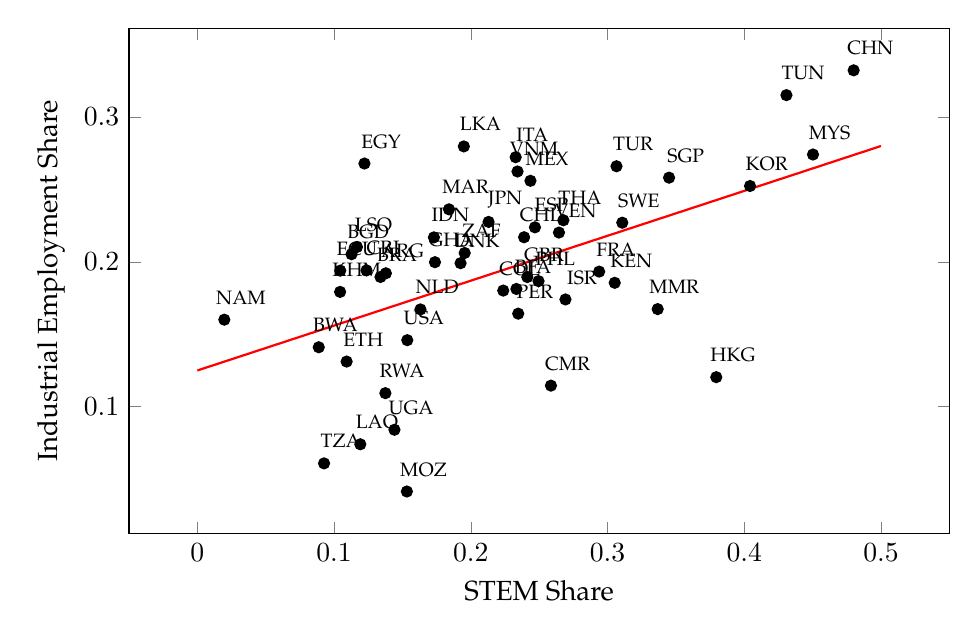
\begin{tikzpicture}
  \begin{axis}[
    width=12cm,
    height=8cm,
       % title={Relationship between STEM Share and Industrial Employment},
    xlabel={STEM Share},
    ylabel={Industrial Employment Share},
    ytick distance=0.1,  
    enlargelimits=0.1,
    scatter/classes={
        a={mark=o,draw=blue}
    },
    every node near coord/.append style={font=\scriptsize} % smaller font for country labels
  ]

    % Scatter points with country names as labels
  \addplot[
  scatter,
  only marks,
  scatter src=explicit symbolic,
  nodes near coords,
  nodes near coords align={center},
  nodes near coords style={font=\scriptsize, yshift=8pt, xshift=6pt} % shift label above marker
]
    coordinates {
 (0.1378744,0.1921153)[ARG]
  (0.2333404,0.1812904)[BFA]
  (0.1127611,0.2052854)[BGD]
  (0.1339324,0.1895628)[BRA]
  (0.0887872,0.1410377)[BWA]
  (0.2389722,0.217)[CHL]
  (0.48,0.3322481)[CHN]
  (0.2586084,0.1145408)[CMR]
  (0.223719,0.1801721)[COL]
  (0.1237097,0.194118)[CRI]
  (0.1925061,0.1990896)[DNK]
  (0.1045007,0.193951)[ECU]
  (0.122197,0.2678931)[EGY]
  (0.2469077,0.223834)[ESP]
  (0.1091694,0.1311437)[ETH]
  (0.2938787,0.1932734)[FRA]
  (0.2413404,0.1895179)[GBR]
  (0.1737703,0.1997761)[GHA]
  (0.3795342,0.1203752)[HKG]
  (0.1730061,0.2169031)[IDN]
  (0.2692143,0.1740516)[ISR]
  (0.2328073,0.2722787)[ITA]
  (0.213,0.2275904)[JPN]
  (0.3052545,0.1855444)[KEN]
  (0.104402,0.1792649)[KHM]
  (0.4042146,0.2523832)[KOR]
  (0.1191805,0.0740409)[LAO]
  (0.1948983,0.2797219)[LKA]
  (0.116723,0.2102498)[LSO]
  (0.1840243,0.2362694)[MAR]
  (0.2436201,0.2559769)[MEX]
  (0.336678,0.1673723)[MMR]
  (0.1532314,0.0414321)[MOZ]
  (0.4502603,0.2741223)[MYS]
  (0.0197044,0.1600689)[NAM]
  (0.1631535,0.1671708)[NLD]
  (0.2346783,0.1642373)[PER]
  (0.2495234,0.1866893)[PHL]
  (0.1375139,0.1093415)[RWA]
  (0.3450148,0.2581424)[SGP]
  (0.3107809,0.2270485)[SWE]
  (0.2676974,0.228728)[THA]
  (0.4308376,0.3151194)[TUN]
  (0.3065551,0.2660213)[TUR]
  (0.0926554,0.0608464)[TZA]
  (0.1441461,0.0840602)[UGA]
  (0.1535388,0.1459264)[USA]
  (0.2644799,0.2202186)[VEN]
  (0.2341544,0.2624081)[VNM]
  (0.1955149,0.206129)[ZAF]
    };

    % Trend line (replace slope/intercept with your regression results)
    \addplot[red, thick, mark=none, domain=0:0.5] {0.31*x + 0.125};
   % \addlegendentry{Trend line (yhat)}

  \end{axis}
\end{tikzpicture}

    \begin{minipage}{0.7\textwidth}  % Adjust width to match figure
        \footnotesize
        \textbf{Note:} STEM share is calculated as the annual number of tertiary graduates in STEM fields divided by total number of tertiary graduates. Industrial employment share is calculated as the number of employees in the industry sector divided by total employment.
    \end{minipage}
    
\end{figure}

%\begin{figure}[h]
%  \centering
%  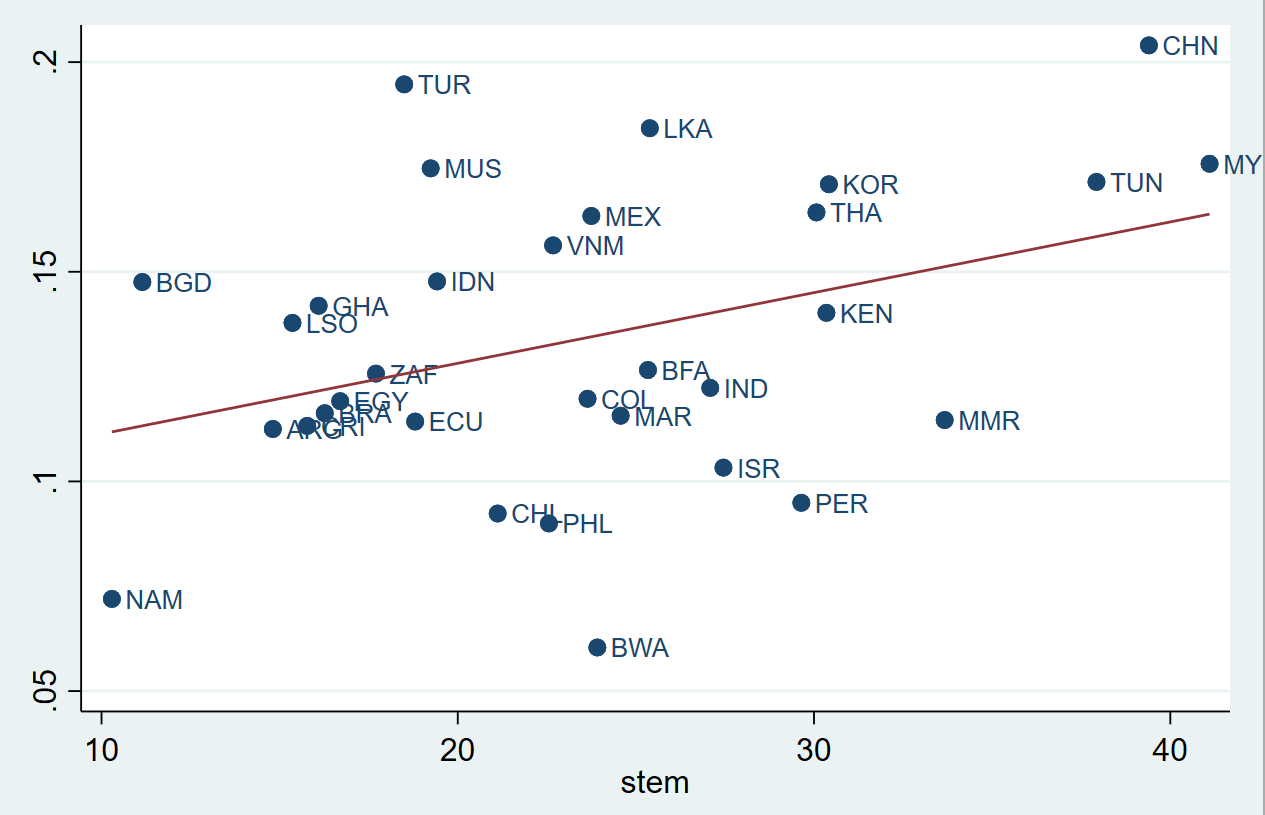
\includegraphics[width=0.8\textwidth]{figures/empirics.png}
%  \caption{Positive relationship between manufacturing employment share and STEM graduate share across 31 emerging economies.}
%  \label{fig:empirics}
%\end{figure}




%The hump-shape relationship between industrial employment and income levels is well discussed in the structural change literature (e.g., \cite{Rodrik2016}. In addition, \cite{huneeus2024heterogeneous} shows a negative relationship between agricultural and industrial employment shares. We further control education attainment  because $STEM_i$ measures only the fraction of potential high-skill workers who choose to study STEM fields, without capturing overall improvements in education attainment. 

The estimates in Table \ref{tab:industry_reg} show a positive and statistically significant correlation between STEM graduate shares and industrial employment shares. In columns (1) and (3),  $\beta_{STEM_i}$ is significant at the 1 percent level: a 1 percentage point increase in STEM share is associated with a 0.24-0.30 percentage point rise in industrial employment share. The coefficient on overall educational attainment is small and negative, suggesting that variation in the composition of tertiary graduates is more closely associated with industrial employment than educational attainment alone. 

\textbf{Correlation and causality.} As will become clearer in the next section, our model is built on the premise that sectoral specialization and skill supply are jointly determined:  countries with a larger industrial sector tend to attract more talent into STEM fields, which we use as a proxy for industrial sector-related skill supply, while a stronger STEM talent pipeline may  support a larger industrial sector. Therefore, the purpose of Figure 1 and Equation \eqref{regression} is to document this relationship as a correlation, rather than to establish a causality. That said, we take a modest step towards exploring the direction of the relationship by   
 re-estimating Equation (\ref{regression}) using only  the subsample of countries for which STEM share data are available at least 5 prior to the employment data. As presented  in Column (2), the coefficient on $STEM_i$ remains significant at the 1 percent level. While this exercise does not resolve concerns about omitted variables or endogeneity, it suggests that the positive association is not  driven solely by contemporaneous correlation and is consistent with a causal interpretation. 


%shows that The preliminary results suggest that the share of STEM graduates is strongly and positively associated with the size of the manufacturing sector. The estimated coefficient on the STEM graduate share, $\alpha_1$, is positive and statistically significant at the 2 percent level, while the coefficient on tertiary attainment, $\alpha_2$, is statistically insignificant. These findings imply that, conditionaif wl on overall tertiary education levels, a higher share of STEM graduates is strongly linked with a larger manufacturing sector, whereas general tertiary attainment alone does not appear to matter.  

\begin{table}[H]
\centering
\begin{threeparttable}
\caption{Dependent Variable: Industrial Employment Share}
\label{tab:industry_reg}
\begin{tabular*}{\textwidth}{@{\extracolsep{\fill}}lccc}
\toprule
                    & (1) All & (2) Sub Sample & (3) All  \\
\midrule
STEM share ($STEM_i$)         & 0.24$^{***}$ & 0.19$^{**}$  & 0.30$^{***}$ \\
                    & (0.07)       & (0.08)       & (0.08)      \\
Edu. attainment     & -0.001$^{***}$ & -0.000$^{**}$ & -0.001     \\
                    & (0.00)       & (0.00)       & (0.00)     \\
Agricultural emp.\ share
                    & -0.20$^{***}$ & -0.18$^{***}$ & --         \\
                    & (0.04)       & (0.05)       &           \\
Log income          & --           & --           & 0.02$^{***}$ \\
                    &             &             & (0.01)    \\
Constant            & 0.23$^{***}$ & 0.21$^{***}$ & -0.03     \\
                    & (0.03)      & (0.03)      & (0.07)    \\
\midrule
Observations        & 50          & 31          & 50        \\
R$^{2}$             & 0.60        & 0.52        & 0.34      \\
\bottomrule
\end{tabular*}
\begin{tablenotes}[flushleft]
\footnotesize
\item Note: The "Sub Sample" includes only economies with STEM share data available at least 5 years  prior to the employment share data. 
Robust standard errors in parentheses.
$^{*}p<0.10$, $^{**}p<0.05$, $^{***}p<0.01$.
\end{tablenotes}
\end{threeparttable}
\end{table}












\section{Model}\label{section model}


\subsection{Environment and timing}
We study a small open economy with two sectors: manufacturing ($m$) and services ($s$). Time is continuous and discounted at rate $r>0$. A unit mass of risk-neutral workers and a continuum of risk-neutral firms populate the economy. Workers choose  sector-specific educational tracks and then search for jobs in the corresponding sector.
In each sector, jobs are formed with DMP-type search and matching frictions.   Let $L_m$ and $L_s$ denote the masses of workers who have acquired the skills relevant for sectors $m$ and $s$, respectively. Thus, $L_i$ is the measure of  the labor force in sector $i$.
The total labor force in the two sectors is fixed at $L$: $L = L_m+L_s$, while the allocation across sectors is endogenous. %An exogenous mass $L_a$ of workers is employed in agriculture sector, hence the total active labor force in $m$ and $s$ sectors is $1-L_a$. 
Let unemployment within sector $i$ be $u_i \equiv L_i-n_i$, where $n_i$ stands for employment in sector $i$. 



\subsection{Preferences, prices, and trade.} 

Employed workers consume a composite  of manufacturing and service goods:\footnote{Here we assume individual workers are grouped into households, and employed members within the same household can pool their consumption, so that every employed member's consumption level would be identical ($c^E$). This assumption helps us avoid distinguishing between the consumption of workers having a manufacturing jobs and of workers with services jobs.}
\begin{equation}
    c^E = (c^E_m)^{\alpha} (c^E_s)^{1-\alpha}.
    \label{eq:ce}
\end{equation}

Unemployed workers receive a flow payoff $z$, which can be interpreted as the value of nonmarketable home production. 

\paragraph{Aggregation.} Let $n$ denote total manufacturing and service employment. Let $C_i$ denote aggregate consumption of good $i$. Aggregate consumption satisfies
\begin{align*}
     n c_m^E & \equiv C_m, \nonumber \\
     n c_s^E &\equiv C_s, \nonumber,  \\
    nc^E &= n   (c^E_m)^{\alpha} (c^E_s)^{1-\alpha}\\
     & =  C_m^{\alpha} C_s^{1-\alpha}.
\end{align*}


Hence,  we can define the aggregate final consumption as 
\begin{equation}
    C \equiv  C_m^{\alpha} C_s^{1-\alpha}.
    \label{eq:finalC}
\end{equation}


We therefore only need to keep track of aggregate consumption  $C_m$, $C_s$ and $C$ in equilibrium.  The unit price of final consumption  is:  
\begin{equation}
    P =  \alpha^{-\alpha}(1-\alpha)^{-(1-\alpha)}  P_m^{\alpha}P_s^{1-\alpha}. \label{eq:P_index}
\end{equation}



Manufacturing goods are fully tradable and  are perfectly substitutes for foreign-produced manufacturing goods.  Hence, the price of domestic manufacturing goods equals the world price : $P_m=p_m=p^F_m$. We set $p^F_m = 1$ as the numeraire.  
The service composite $C_s$ is a CES aggregate of domestically produced $C_s^H$ and imported services $C_s^F$ with elasticity of substitution $\nu$:
\begin{equation}
C_s=\Big[\chi (C_s^H)^{\frac{\nu-1}{\nu}} + (1-\chi)\,(C_s^{F})^{\frac{\nu-1}{\nu}}\Big]^{\frac{\nu}{\nu-1}},
\quad \chi \in(0,1).
\label{eq:ces_services}
\end{equation}
 where $1-\chi$ governs the service-trade openness , and  $\nu>1$ implies that foreign and domestic services are gross substitutes.  The import price of services is exogenous at $p_s^F$. The domestic service price $p_s$ is endogenous in equilibrium.  The unit price of the service composite is:
\begin{equation}
P_s=\Big[\chi \,p_s^{\,1-\nu} + (1-\chi)\,(p_s^{F})^{1-\nu}\Big]^{\frac{1}{1-\nu}},
\label{eq:Ps_index}
\end{equation}
 
 \paragraph{Trade pattern.} We assume that the home country has a comparative advantage in manufacturing relative to the rest of the world: $p_s/p_m > p_s^F/p_m^F=1$. Therefore, the economy is a net exporter of manufacturing goods and a net importer of services. We assume balanced trade in every period. 

 \paragraph{Consumption demand.} Let total nominal expenditure be $E\equiv PC$. Standard utility maximization implies the following consumption demands:

 \begin{align}
C_m  &=   \frac{\alpha}{p_m}E,  \label{eq:Cm}  \\
C_s &= \frac{1-\alpha}{P_s}E, \\
C_s^{H} &  = \chi \left(\frac{p_s}{P_s}\right)^{-\nu} C_s, \\
C_s^{F} &  = (1-\chi) \left(\frac{p^F_s}{P_s}\right)^{-\nu} C_s.  \label{eq:CsF_def}
\end{align}

 




\subsection{Labor market and production}

Labor markets in manufacturing and services are segmented. Each sector $i \in \{m, s\}$ operates a  labor market with DMP-style search and matching frictions.  Each job consists of a one-vacancy-one-worker pair. Let $u_i$ and $v_i$ denote the masses of unemployed workers and unfilled vacancies in sector $i$.  Matches are formed according to  
\begin{align}
    m_i=M(u_i,v_i).
\end{align}
The matching function $M(\cdot, \cdot)$  is increasing, concave, and homogeneous of degree one.  In the quantitative exercise section, we assume
\begin{align}
    M(u_i,v_i)= u_i^\eta v_i^{1-\eta},
\end{align}
where $\eta\in (0,1)$ is the elasticity of matches with respect to unemployment. Define market tightness as
\begin{align}
    \theta_i\equiv v_i/u_i.
\end{align}
The vacancy–filling rate is then
\begin{align}
    q_i(\theta_i)\equiv M_i(u_i,v_i)/v_i,
\end{align}
and the job–finding rate is
\begin{align}
    \theta_i q_i(\theta_i)\equiv M_i(u_i,v_i)/u_i.
\end{align}




\paragraph{Job-specific capital and production.}
 Creating a vacancy in sector $i$ requires installing job–specific capital $k_i\ge 0$. Once chosen, the capital level cannot be changed until the capital depreciates and the vacancy is destroyed. Because capital is sunk at the time of wage bargaining, it generates a holdup problem.  
Once a vacancy is filled, the match produces output at rate $f_i(k_i)$ with $f_i'>0$, $f_i''<0$, and $f_i(0)=0$. %Let total  employment in sector $i$ be $n_i$, which has to equal the difference between total labor force and unemployment in the sector:  $n_i=L_i-u_i$. 
Total output in sector $i$ is thus the product of per-match output and employment:
\begin{equation}\label{eq:Y_i}
    Y_i= f_i(k_i)n_i, \qquad i\in\{m,s\}.
\end{equation}

Following \cite{acemoglu1999holdups}, we assume that the job-specific capital attached to any vacancy, filled or unfilled, is lost with exogenous Poisson probability $s_i$, at which point the match is also separated.\footnote{Allowing $s_i$ to differ by sector helps reconcile two empirical regularities: (i) manufacturing and services exhibit similar or slightly lower \emph{unemployment rates} in manufacturing, $\bar u_m \lesssim \bar u_s$, where $\bar u_i\equiv u_i/L_i$; (ii) manufacturing is more capital intensive. Higher $k_m$ raises hold–up costs and would otherwise push $\bar u_m$ above $\bar u_s$; taking $s_m<s_s$ captures longer job durations in capital–intensive matches and restores consistency with the data without inflating education costs or wages.} 

\paragraph{Employment and unemployment dynamics.}
 Employment evolves according to:
\begin{align}
    \dot{n}_i = m_i -s_in_i,  \qquad i\in\{m,s\}.
\end{align}
 Within each sector, 
 \begin{align}
     u_i &= L_i-n_i,\\
     v_i & = \theta_i u_i.
 \end{align}
 Let $x_i$ denote the flow of new vacancies created, vacancy dynamics thus satisfy
 \begin{align}
  %  \dot{n_i}(t) &= m_i(t) - s_in_i(t), \\
  %  m_i(t) &= q_i(\theta_i)\theta_iu_i(t),\\
  %  u_i(t) &= L_i(t)-n_i(t),\\
  %  v_i(t) &= \theta_iu_i(t),\\
    \dot{v_i} &= x_i- s_iv_i- m_i.
\end{align}

\noindent Unemployment dynamics are given by
\[
\dot u_i = s_i(L_i-u_i)-\theta_i q_i(\theta_i)u_i.
\qquad i\in\{m,s\},
\]
In steady state, the unemployment \emph{rate}  $\bar u_i\equiv u_i/L_i$ is given by 
\begin{equation}\label{u_dynamics}
u_i^{ss}=\frac{s_i}{s_i+\theta_i q_i(\theta_i)}\,L_i,
\qquad
\bar u_i^{ss}=\frac{u_i^{ss}}{L_i}=\frac{s_i}{s_i+\theta_i q_i(\theta_i)}.
\end{equation}






\paragraph{Education and workers' sectoral choices.}
Before entering the labor market, workers choose which sector-specific skills to acquire and this choice is permanent.  
Acquiring the skills for sector $i$ requires a one-time training cost $\epsilon_i$, measured in units of the final consumption good.  We assume $\epsilon_m \geq \epsilon_s$, reflecting the idea that manufacturing-related skill training is  typically more costly than service-related skill training.  %Workers differ in their ability to acquire manufacturing-suitable skill and we denote this heterogeneity as a cost function $c(j)$ that is increasing in $j$.  
%Let $J^U_m$ and $J^U_s$ denote the expected life-time value of an unemployed worker in manufacturing and services, respectively. %In equilibrium, $J^U_m - J^U_s$ must hold so that there is an interior solution for $L_m$ and $L_s$.


%The total size of labor force is $1$. A share $L_a \in (0,1)$ of the labor force is exogenously employed in agriculture.  Agricultural workers do not participate in  manufacturing or service labor markets. In equilibrium, the size of workforces who choose manufacturing (services) training and hence enter the job market of manufacturing (service) is constrained by total non-agriculture job supply:
%\begin{equation}\label{eq:L_m+L_s}
%    L_m+L_s=\bar{L}=1-L_a. 
%\end{equation}




\subsection{Bellman equations and definition of decentralized equilibrium}\label{sec:DE}






Let $J_i^U$ and $J_i^E(k_i)$ denote a worker’s values of unemployment and employment in sector $i$, and let $J_i^V(k_i)$ and $J_i^F(k_i)$ denote a firm’s values of a vacancy and a filled job. Here, $J^V_i(k_i)$  is  the value of a vacancy before netting out the capital installation cost. A firm that creates a vacancy with capital $k_i$ therefore earns a net value  $J^V_i(k_i) - P_kk_i/P$ measured in units of the final consumption good. 
The corresponding Bellman equations are:

\begin{align}
rJ_i^U &= z + \theta_i q_i(\theta_i)\big(J_i^E(k_i^*)-J_i^U\big), \label{eqn:U_bell}\\
rJ_i^E(k_i) &= \frac{w_i(k_i)}{P} + s_i\big(J_i^U-J_i^E(k_i)\big), \label{eqn:E_bell} \\ 
rJ_i^V(k_i) &=  q_i(\theta_i)\big(J_i^F(k_i)-J_i^V(k_i)\big) - s_i J^V_i(k_i), \label{eqn:V_bell}\\
rJ_i^F(k_i) &= \frac{p_i f_i(k_i) - w_i(k_i)}{P} - s_i J_i^F(k_i), 
\label{eqn:F_bell} \\
%J_i^V&= \max_{k_i} \{ J_i^V(k_i) \}
\text{where }k_i^{*}
&= \operatorname*{arg\,max}_{k_i}\left\{ J_i^{V}(k_i) - \frac{P_k\,k_i}{P} \right\}.
\label{eqn:kstar}
\end{align}

Equation (\ref{eqn:U_bell}) gives the flow value of an unemployed worker  in sector $i$: the unemployment income  plus the expected payoff from   finding a job. We model unemployment income as home production of  $z$,  measured in units of  final consumption good. %\footnote{This characterization of home production as service goods is not new in the literature, for example, in \cite{moro2017does}.}  
The expected gain from  finding a job equals the job finding rate $\theta_i q_i (\theta_i)$ times the gain from employment, $J_i^E(k^*)-J^U_i$ where $k_i^*$ denotes the equilibrium level of capital per worker in sector $i$. Equations (\ref{eqn:E_bell}) gives the flow value of an employed worker in sector $i$ conditional on the job's capital level $k_i$, taking into account the real wage $w_i(k_i)/P$ and the separation rate $s_i$. Equation (\ref{eqn:V_bell}) gives the flow value of a vacancy with capital level $k_i$, which includes the expected gain from the vacancy being filled and the expected loss from the destruction of the vacancy. The level of $k_i$ is optimally chosen by firms to maximize the value of the vacancy. Finally, (\ref{eqn:F_bell})  gives the flow value of a filled job with capital $k_i$: the firm receives real output $p_if_i(k_i)/P$, pays labor $w_i(k_i)/P$, and accounts for the separation rate $s_i$.





\paragraph{Capital choice (holdup).}
The firm chooses the capital level when the vacancy is created. Once the vacancy is created,  the capital cost becomes sunk. The firm therefore chooses capital to maximize its expected profit $J^V_i(k_i) - \frac{P_kk_i}{P}$.



\paragraph{Wage bargaining.} After a worker is matched with a vacancy, the wage is determined through Nash bargaining, with the worker's bargaining weight given by $\beta\in(0,1)$:
\begin{equation}\label{eq:nash}
(1-\beta)\big(J_i^E(k_i)-J_i^U\big)=\beta\big(J_i^F(k_i)-J_i^V\big).
\end{equation}


\paragraph{Free entry condition.} Free entry by firms implies that the expected equilibrium profit from creating a vacancy is zero:
\begin{equation}\label{eq:JV=0}
    J_i^V(k^*_i) =\frac{P_kk^*_i}{P}. 
\end{equation}

\paragraph{Workers' sectoral choice.} In equilibrium, workers are indifferent between entering the manufacturing or service markets:
\begin{equation}
    J^U_m - J^U_s = \epsilon_m-\epsilon_s \label{eq:JUm=JUs}
\end{equation}








\paragraph{Definition of decentralized equilibrium.}

A stationary decentralized equilibrium (DE) consists of

(i) Prices $(p_s, P_s, P)$, 

(ii) Sectoral labor market  objects $\{  L_i, \theta_i, u_i, n_i, v_i, k_i, w_i            \}_{i\in  \{m, s\} }$, and

(iii) Good market quantities 
$\{E, C_m, C_s, C^H_s, C^F_s, X_m, M_s\}$, 


Such that:

1. Given prices $(p_m, p_s, p_s^F)$ and total expenditure $E$, consumption demands satisfy \eqref{eq:Cm} - \eqref{eq:CsF_def}. 

2. Firms and workers' optimize  in  the labor market, so that the value functions satisfy \eqref{eqn:U_bell}- \eqref{eqn:kstar} and wages $w_i(k_i)$ satisfies Nash bargaining \eqref{eq:nash}.

3. Free entry of firms characterized  by \eqref{eq:JV=0}.

4. Workers' sectoral choices satisfy  \eqref{eq:JUm=JUs}. 

5. Total labor supply satisfies $L_s+L_m = L$.

6. Production  satisfies $Y_i = f_i(k_i)n_i$.  


7. Good markets are clear and trade is balanced, as in \eqref{eq:m_clearing} - \eqref{eq:tradebalance}, and 

8. Labor market flows satisfy \eqref{u_dynamics}.
 

\subsection{Characterization of the Decentralized Equilibrium}

We characterize the stationary decentralized equilibrium in two blocks. 
\begin{itemize}
    \item A \textit{goods market block} maps $(Y_m, Y_s, I)$ into the equilibrium domestic service price $p_s$ consistent with household utility maximization, market clearing, and balanced trade. This mapping is independent of the structure of labor market.  

    \item A \textit{labor market block} maps $p_s$ into labor market outcomes $(\theta_i, k_i, w_i, n_i, L_i)$, and therefore into ($ Y_m, Y_s, I)$. 
    
    The decentralized equilibrium is a fixed point of these two mappings. 

\end{itemize}





\subsubsection{Goods market equilibrium block}
This block derives the equilibrium domestic service price $p_s$, as well as consumption and trade flows, given foreign prices  $(p_m^F, p_s^F)$, real output  $(Y_m, Y_s)$, and nominal investment $I$.




\paragraph{Goods-market clearing and balanced trade.}  In the market for manufacturing goods, total output must equal  the sum of domestic consumption, investment, and exports: 
\begin{equation}
    Y_m = C_m + I + X_m. \label{eq:m_clearing}
\end{equation}
Total investment is given by
\begin{equation}
    I = P_k(x_mk_m+x_sk_s),  \label{eq:capital_cost}
\end{equation}
where $x_i$ denotes the flow of newly created vacancies in sector $i$.\footnote{At steady state, the number of vacancies created in each moment should equal the number of vacancies destroyed: $x_i = s_i(n_i+v_i)$.}

For services, 
\begin{align}
    C_s^H &= Y_s,  \label{eq:CsH}\\
    C_s^F & = M_s.  \label{eq:CsF}
\end{align}

Trade is balanced:
\begin{equation}
    p_m X_m = p^F_sM_s.   \label{eq:tradebalance}
\end{equation}


Nominal GDP is defined as 
\begin{equation}
    Y^N = p_mY_m + p_sY_s.
\end{equation}


Total nominal consumption expenditure

\begin{align}
    E \equiv PC &\equiv p_m C_m + p_sC^H_s + p_s^FM_s \\
   &  = p_m(Y_m-I) + p_sY_s,   \label{eq:E}
\end{align}
where the last equality  uses \eqref{eq:m_clearing} - \eqref{eq:tradebalance}.


\begin{proposition}\label{prop:tradeblock}
    Given exogenous prices $p_m, p_s^F $, output $(Y_m, Y_s)$, and investment $I$, the  domestic service price $p_s(p_m, p_s^F, Y_m, Y_s, I)$ is determined by
\begin{equation}
Y_s
=
\chi (1-\alpha)\,\big(p_m (Y_m-I) + p_s Y_s\big)\, p_s^{-\nu}\, P_s^{\nu-1},
\label{eq:ps_solution}
\end{equation}
where $P_s$ is given by \eqref{eq:Ps_index}.  

Given $p_s$, the final-good price $P$ and  nominal consumption $E$ are determined by \eqref{eq:P_index} and \eqref{eq:E}. Consumption allocations  are determined by \eqref{eq:Cm}-\eqref{eq:CsF_def}. Exports $X_m$ and imports $M_s$ are pinned down by \eqref{eq:CsF} and \eqref{eq:m_clearing}.
\end{proposition}





\subsubsection{Labor market equilibrium block}


From \eqref{eqn:V_bell} and \eqref{eqn:F_bell}, we have
\begin{align}
    J_i^F(k_i) &=   \frac{p_i f(k_i)-w_i(k_i)}{P(r+s_i)},\\
    J_i^V(k_i) & =   \frac{q_i(\theta_i)}{r+s_i+q_i(\theta_i)}J_i^F(k_i).  \label{eq:JV_int1}
\end{align}

A firm chooses $k_i$ to maximize its expected profit $J^V_i(k_i)- P_kk_i/P$.  The first-order condition is therefore
\begin{align}
        P_k &= \frac{q_i(\theta_i)}{r+s_i+q_i(\theta_i)} \frac{p_i f'(k_i) - w_i'(k_i)}{r+s_i}.  \label{eqn:P_k_w}
\end{align}


From  \eqref{eqn:E_bell} and  \eqref{eqn:V_bell} , we have
\begin{align}
    \frac{p_i f(k_i)-w_i(k_i) }{P}
    & = \frac{(1-\beta_i)\big(r+s_i+q_i(\theta_i)\big)}{\,r+s_i+(1-\beta_i)q_i(\theta_i)\,}\big[\frac{p_i f(k_i)}{P}-rJ_i^U\big].
\end{align}

Substitute it into \eqref{eqn:P_k_w}, we have the optimality condition for $k_i$:
\begin{equation*}
 %\boxed{
     P_k  = \frac{q_i(\theta_i)(1-\beta_i)}{r+s_i}\,\frac{p_i f'(k_i)}{\,r+s_i+(1-\beta_i)q_i(\theta_i)\,}.
%}   
\end{equation*}

\noindent \textbf{Total surplus $S_i(k_i)$:} To build intuition, it is useful to define the total surplus of a match in 
in sector $i$ as
\[
S_i(k_i) \;\equiv\; (J_i^E(k_i)-J_i^U) + (J_i^F(k_i)-J_i^V(k_i)).
\]

Nash bargaining in \eqref{eq:nash} then implies
\begin{equation} \label{partial_surplus}
    J^E_i-J^U_i = \beta S_i, \quad J^F_i-J^V_i = (1-\beta)S_i .
\end{equation}

Using \eqref{eqn:U_bell}–\eqref{eqn:F_bell}, we obtain:
\begin{equation}
    r(J^E_i(k_i)-J^U_i) = \frac{w_i(k_i)}{P} -z- (s_i+\theta_iq(\theta_i))(J^E_i(k_i)-J^U_i),
\end{equation}
\begin{equation}\label{eq:JF-JV}
    r(J^F_i(k_i)-J^V_i(k_i)) = \frac{p_if_i(k_i) -w_i(k_i)}{P}  - (s_i+q(\theta_i))(J^F_i(k_i)-J^V_i(k_i)).
\end{equation}
Adding these two equations and using \eqref{partial_surplus}, we get
%\begin{equation*}
%    (r+s_i)S_i = p_iA_i\phi_i(k_i) -\theta_iq(\theta_i)\beta S_i - q(\theta_i)(1-\beta)S_i,
%\end{equation*}
%Hence 
\begin{equation}\label{eq:Si}
S_i(k_i)\;=\;\frac{p_if_i(k_i)/P-z}{D_i(\theta_i)}, \label{eq:Si(k)}
\end{equation}
where
\begin{equation}\label{eq:Di}
D_i(\theta_i)\;\equiv\; r+s_i+(1-\beta)\,q_i(\theta_i)+\beta\,\theta_i q_i(\theta_i).  \label{eq:Di}
\end{equation}


Thus, the total surplus of match in sector $i$ equals the output flow net of home production, discounted by $D_i$. The discount term $D_i$ reflects the time discount rate $r$, the separation rate $s_i$, and the adjustment due to the transitions between vacancies and matches and between unemployment and employment.  Note that the sunk capital cost $P_kk_i$ does not enter $S_i(k_i)$  because capital investment happens before  wage bargaining. 


The other two key equilibrium conditions are the free-entry condition  \eqref{eq:JV=0} and the workers' sectoral choice condition \eqref{eq:JUm=JUs}. Given total match surplus $S_i(k_i)$, the value of a vacancy $J^V_i(k_i)$ and the value of unemployment $J^U_i$  follow directly from \eqref{eqn:U_bell}, \eqref{eqn:V_bell} and Nash bargaining:
\begin{align}
    J^V_i(k_i) &= \frac{q_i(\theta_i)(J^F(k_i)-J_i^V(k_i))}{r+s_i} = \frac{q_i(\theta_i)(1-\beta)S_i(k_i)}{r+s_i}, \\
    J^U_i &= \frac{\theta_iq_i}{r}(J^E_i(k^*_i)-J^U_i) = \frac{\beta\theta_iq_i}{r}S_i(k_i^*).
\end{align}

\begin{proposition}[Decentralized equilibrium]
\label{prop:DE}


In steady state, the decentralized equilibrium  $(k^*_i, \theta^*_i, L^*_s)$  is characterized by the following conditions:

\begin{align}
%\boxed{%
\{\text{Capital choice}\}&:  P_k  = \frac{q_i(\theta_i)(1-\beta)}{r+s_i}\,\frac{p_i f'(k_i)}{\,r+s_i+(1-\beta)q_i(\theta_i)\,},  
\qquad i\in\{m,s\};
\label{eq:DE_char_cap_main}\\
\{ \text{Tightness} \}&:  \frac{P_{k} \, k_i }{P}
= \frac{q_i(\theta_i)(1-\beta)}{r+s_i} \;
  \frac{p_i f_i(k_i)/P-z}
       {D_i(\theta_i)}, \qquad i\in\{m,s\};
\label{eq:DE_char_theta_main}\\
\{\text{Sectoral choice}\}&: r(\epsilon_m-\epsilon_s)
= \frac{\beta\,\theta_m q_m(\theta_m)}{D_m(\theta_m)}\,[p_m f_m(k_m)/P- z]
-\frac{\beta\,\theta_s q_s(\theta_s)}{D_s(\theta_s)}\,[p_s f_s(k_s)/P- z], \label{eq:DE_char_edu_main}
%\text{where} %& \quad 
  %  D_i(\theta_i) = r+s_i + (1-\beta_i) q_i(\theta_i) + \beta_i \theta_i q_i(\theta_i). \label{eq:DE_Di}
\end{align}
%where $D_i(\theta_i)$ is defined in \eqref{eq:Di}.

\end{proposition}



\paragraph{Remarks.}  
  Equation \eqref{eq:DE_char_cap_main} determines firms' optimal capital choices. The left-hand side is the rental cost of capital required to create or maintain a vacancy. The right-hand side captures the marginal life-time return from additional investment.  The term $\frac{p_if_i'(k_i)}{r+s_i+(1-\beta_i)q_i(\theta_i)}$ captures the marginal increase in  surplus from higher capital.\footnote{The denominator $r+s_i+(1-\beta_i)q_i$ differs from $D_i$ in \eqref{eq:Si(k)} and \eqref{eq:Di}. The derivation of \eqref{eq:DE_char_cap_main} takes $J^U_i$ as given because it is an equilibrium outcome. The derivation of  \eqref{eq:Si(k)} and \eqref{eq:Di} takes into account that a change $k_i$ can also affect $J^U_i$ in equilibrium.  }  This flow return is discounted by interest rate and separation rate, $(r+s_i)$, and is adjusted for the vacancy filling rate, $q_i(\theta_i)$. Importantly, the  $(1-\beta)$ term captures the  \emph{capital holdup problem} highlighted in \cite{acemoglu1999holdups} and \cite{cardullo2015sunk}: firms internalize only a fraction of the match surplus when they choose $k_i$, leading to under–investment relative to the social planner's allocation which we characterize in the next section. 
  
Equation \eqref{eq:DE_char_theta_main} reflects the free-entry condition %\eqref{eq:JV=0} 
in equilibrium. A firm creates a vacancy at cost $P_k k_i/P$, and its return is $1-\beta$ share of total surplus flow. This surplus flow is converted to a life-time value by discounting at $r+s_i$ and adjusting for the vacancy filling rate.


Equation \eqref{eq:DE_char_edu_main} governs workers' sectoral  choices. The left-hand side is the training cost differential, while the  right-hand side
captures the difference in workers' expected surpluses from entering each sector. The expected surplus from entering sector $i$ is given by the worker's bargaining share $\beta$, times  the job-finding rate $\theta_i q_i (\theta_i)$ and total surplus $S_i$. 






% ===============================================================

\section{Social Planner’s (SP) Problem}
\label{spp analysis}
% ===============================================================

%Now, we move on to characterize the social planner's problem. For each sector $i \in \{s,m\}$ define: 

%\begin{itemize}
%  \item $m_i(t)$: newly formed matches at time $t$;
%  \item $v_i(t)$: (unfilled) vacancies at time $t$;
%  \item $n_i(t)$: employment at time $t$;
 % \item $L_i(t)$: exogenous labor endowment in sector $i$, with $L_s + L_m = L$ and $L_m = L - L_s$;
%  \item $q_i(\theta_i)$: meeting rate per vacancy as a function of market tightness $\theta_i$;
%  \item $\theta_i(t)$: labor market tightness in sector $i$, so that $v_i(t) = \theta_i(t)\bigl(L_i(t) - n_i(t)\bigr)$.
%\end{itemize}

Let $\mathcal{C}(Y_m, Y_s, I)$ denote the level of final consumption implied by the goods-market equilibrium for given output $(Y_m Y_s)$ and investment  $I$, as characterized by Proposition \ref{prop:tradeblock}. The social planner chooses $\{ \theta_i(t), k_i(t), L_s(t) \}_{t \ge 0}$ to maximize the present discounted value of output net of capital and education costs:\footnote{Note that skill acquisition cost $\epsilon_i$ in the model is incurred once when workers choose a sector. In the planner's objective function, we can represent this one-time cost in an equivalent flow term $r\epsilon_i$ because $\int_0^{\infty}  re^{-rt}dt=1$. }



\begin{align}
\max_{\{\theta_i,\,k_i,\,L_s\}}
\int_{0}^{\infty}
\Bigl\{
%p_mY_m/P+p_sY_s/P +z(u_s+u_m) - \sum_{i\in \{m, s\}} [m_i(t) (r+s_i)v_i(t)]P_kk_i(t)/P
\mathcal{C}(Y_m(t), Y_s(t), I(t)) +z(u_m(t)+u_s(t))
- r\,L_m(t)\epsilon_m - rL_s(t)\epsilon_s
%- r\int_0^{L_m} c(j) di
\Bigr\}
e^{-rt}\,dt,
\label{eq:SPP_AS_two_sectors_objective}
\end{align}
subject to, for each sector $i \in \{s,m\}$,
\begin{align}
    \dot{n}_i(t) & = m_i(t) - s_i n_i(t), \label{eq:ni_law_motion}\\
        \dot{Y}_i(t) & = -s_iY_i(t) + m_i(t)f_i(k_i(t)), \\
        u_i(t) &= L_i(t) - n_i(t), \\
    m_i(t) & = q_i\bigl(\theta_i(t)\bigr)\,\theta_i(t)\,\bigl(L_i(t) - n_i(t)\bigr), \label{eq:mi_def}\\
    v_i(t) & = \theta_i(t)\,\bigl(L_i(t) - n_i(t)\bigr), \label{eq:vi_def}\\
    L_m(t) & = L - L_s(t).
%    Y(t) &= [\alpha Y(t)_m^{\rho} + (1-\alpha Y_s(t)^{\rho}]^{1/\rho}\\
\end{align}
%where $p_s$ is determined by  $F(p_s; Y_m, Y_s, G)=0$ in the trade block and $G=\sum_i s_i(n+v_i)P_kk_i$.


\begin{proposition}[Social Planner]
\label{prop:SPP}
In steady state, the social planner's choices of $k_i$, $\theta_i$ and $L_s$ are characterized by

\begin{align}
%\boxed{%
\{\text{Capital choice}\}&: \quad P_k \;=\; \frac{p_i f'\bigl(k_i\bigr)}{r+s_i}\;\frac{q_i(\theta_i)}{\,r+s_i + q_i(\theta_i)\,}, \quad i\in \{m,s\}   \label{eq:SPP_capital_condition_boxed} \\
\{ \text{Tightness} \}&: \quad \frac{P_k\,k_i}{P}
\;=\;
\frac{q_i(\theta_i)\,(1-\eta)\,(p_i f(k_i)/P-z)}{(r+s_i)D_i(\eta)},  \quad i\in \{m,s\}  \label{eq:SPP_theta_condition_boxed}  \\
\{\text{Sectoral choice}\}&: \quad  r(\epsilon_m-\epsilon_s)
=\theta_m q_m(\theta_m)\,\eta \Phi_m - \theta_s q_s(\theta_s)\,\eta \Phi_s,\label{eq:SPP_Ls_condition_boxed}\\
\nonumber \\
%\frac{ \theta_m q_m(\theta_m)\,\eta_m\, (p_m f_m(k_m)-P_sz) }
%     { D_m^{SP}}
%-
%\frac{ \theta_s q_s(\theta_s)\,\eta_s\, (p_s f_s(k_s)-P_sz) }
%     { D^{SP}_s }
\text{where} & \quad 
    \Phi_i = \frac{p_if_i(k_i)/P-z}{D_i(\eta)},  \label{eq:Phi}\\
   & \quad D_i(\eta) = r+s_i + (1-\eta) q_i(\theta_i) + \eta \theta_i q_i(\theta_i).\\
   & \quad \eta \equiv \frac{\partial log M(u,v)}{\partial log (u)}. %\text{is the elasticity of matches with respect to unemployment}.
\end{align}

\end{proposition}


\paragraph{Remarks.}  
Equation \eqref{eq:SPP_capital_condition_boxed} characterizes the social planner's optimal choice of $k_i$. The right hand side is the marginal social return to capital:  $p_if_i'(k_i)$, the marginal product of capital, discounted by the interest rate and separation rate, and adjusted by the probability that the vacancy is filled,  $\frac{q_i}{r+s_i+q_i}$. Equation \eqref{eq:SPP_theta_condition_boxed} and \eqref{eq:SPP_Ls_condition_boxed} are the planner's counterparts to the decentralized equilibrium conditions \eqref{eq:DE_char_theta_main} and \eqref{eq:DE_char_edu_main}, except that $\beta$ is replaced with $\eta$,   the elasticity of matches with respect to employment. 

The planner internalizes how changes in labor market tightness affect match formation, so the relevant object is the elasticity $\eta$.  In the decentralized equilibrium, however, the corresponding  condition depends on workers' bargaining power $\beta$, which governs how surplus is privately shared. The Hosios condition, $\beta=\eta$, is therefore a natural benchmark: when it holds, the decentralized equilibrium coincides with the planner on search externality, but the capital holdup distortion remains. 


% ---------------------------------------------------------------
\section{Efficiency}
\label{sec:ineff_general}
% ---------------------------------------------------------------

To analyze the sources of inefficiency, we compare the optimality conditions of decentralized equilibrium (DE)  with those of social planner's allocation (SP). Let $\{k_i^{DE}, \theta_i^{DE}, L_i^{DE} \}$ denote the allocation that satisfies DE's conditions \eqref{eq:DE_char_cap_main}-\eqref{eq:DE_char_edu_main}  and 
 $\{k_i^{SP}, \theta_i^{SP}, L_i^{SP} \}$ as bundle satisfying SP's conditions \eqref{eq:SPP_capital_condition_boxed}-\eqref{eq:SPP_Ls_condition_boxed}.


\subsection{Hosios condition $\beta=\eta$.}
%We start by comparing the DE with SPP under the assumption that the Hosios condition $\beta = \eta$ holds for both sectors.

\begin{proposition}\label{prop_efficiency_hosios}
    Under Hosios condition, $\beta=\eta$,
    \begin{enumerate}
        \item[(i)] The decentralized equilibrium is constrained inefficient;
%        conditional the same $\theta_i$ and $L_s$, the equilibrium capital choice $k_i^{DE}(\theta_i, L_s)$ is smaller than socially optimal capital level $k_i^{SP}(\theta_i, L_s)$.\\
        \item[(ii)]  If  $k_i = k_i^{SP}$ is fixed exogenously, then $\theta^{DE}_i = \theta^{SP}_i$ and $L_i^{DE}=L_i^{SP}$. 
    \end{enumerate}
\end{proposition}


%\textcolor{red}{SG note: will have to come back to show the comparison of $k$ and $L_m$ to make it complete.}



\paragraph{Remarks.} Proposition \ref{prop_efficiency_hosios} ($i$) follows directly from comparing the private and social marginal return to  capital in  \eqref{eq:DE_char_cap_main} and \eqref{eq:SPP_capital_condition_boxed}. Define the capital wedge $\Omega_i^K$ as the ratio between  the private and social marginal return to capital:
\begin{align}
\Omega_i^{K} & \equiv\ \frac{\text{Marginal return to  $k$}_i^{DE}}{\text{Marginal  return to $k$}_i^{SP}}  \nonumber\\
 & \equiv \frac{\frac{q_i(\theta_i)(1-\beta)}{r+s_i}\,\frac{p_i f'(k_i)}{\,r+s_i+(1-\beta)q_i(\theta_i)\,}}{\frac{p_i f'(k_i)}{r+s_i}\;\frac{q_i(\theta_i)}{\,r+s_i + q_i(\theta_i)\,}}
\;=\;(1-\beta)\,\frac{\,r+s_i+q_i(\theta_i)\,}{\,r+s_i+(1-\beta)\,q_i(\theta_i)\,}<1.
\end{align}
%Since $\beta_i \in (0,1)$, $q_i(\theta_i) > (1-\beta_i)q_i(\theta_i)$, which implies the fraction is greater than 1. However, since $(1-\beta_i)(r+s_i+q_i(\theta_i)) < r+s_i+(1-\beta_i)q_i(\theta_i)$ (as $-\beta_i(r+s_i) < 0$), we have $\Omega_i^{K} < 1$.
Therefore, the private marginal return to capital in DE is smaller than the social marginal return to capital in SP.   However, when $\beta=\eta$, \eqref{eq:DE_char_theta_main}-\eqref{eq:DE_char_edu_main} in DE are identical to \eqref{eq:SPP_theta_condition_boxed}-\eqref{eq:SPP_Ls_condition_boxed}, which leads to Proposition \ref{prop_efficiency_hosios} (ii). 


\begin{proposition}\label{prop_implementation_hosios}
    Under Hosios condition  $\beta=\eta$ , a deficit-neutral policy consisting of a one-time investment subsidy $\tau^{K*}_i$ per unit of investment and an one-off lump-sum tax on firms $\tau^{T*}_i$ per vacancy implements the social planner's allocation:
\begin{align*}
    \tau_i^{K*} & = 1-\Omega_i^K=  1-\frac{(1-\beta)(r+s_i+q_i(\theta_i^{SP}))}{r+s_i+(1-\beta)q_i(\theta_i^{SP})} >0\\
    \tau_i^{T*} & = - \tau^{K*}P_kk_i^{SP}/P<0
\end{align*}
\end{proposition}



The proof of Proposition \ref{prop_implementation_hosios}   is available in Appendix \ref{appendix:DE_policy}.   
Intuitively, the investment subsidy $\tau^{K*}_i$ corrects the inefficiency arising from capital hold-up and induces firms to choose  higher $k^i$. This subsidy also raises firms' profits, encouraging (inefficiently) more firms to enter. Thus, a lump-sum tax on firm entry, $\tau^T_i$,  is needed to prevent inefficient over-entry. 
Another key implication is that once the capital level is efficient,  there is no need to subsidize workers' trainings as long as Hosios condition holds, as higher per worker capital endogenously raises  workers' incentives to enter the manufacturing sector.  

What are the real-world counterparts of $\tau_i^K$ and $\tau_i^T$? The investment subsidy $\tau_i^K$ maps naturally into policies that reduce  the net cost of investment, such as accelerated depreciation allowances,  investment tax credits, or direct investment subsidies. The counterpart of the lump-sum tax $\tau_i^T$ is more subtle. It is best interpreted as a firm contribution that is proportional to employment but do not vary one-to-one with the total wage bill. Examples include a flat payroll tax, a flat social security contribution, or payroll taxes that apply only up to  low wage threshold.


\subsection{Empirical evidence: skill supply responds to skill demand.}

A key premise of Proposition \ref{prop_implementation_hosios} is that workers' educational choices respond to shifts in skill demand. To illustrate this mechanism empirically, we follow \cite{han2020industry} to use the response of petroleum-engineering enrollment to movements in real oil prices as evidence that skill supply adjusts to demand.  This relationship has several advantages. 
First, real oil price can plausibly be treated as an  exogenous shock to labor demand in the oil industry. When oil prices rise, an increase petroleum-engineering enrollment can be interpreted as a causal  response to this demand shock.  Second, unlike broad fields such as mathematics, petroleum engineering is narrowly defined and closely tied to the oil industry. This tighter mapping helps isolate the demand channel and reduces concerns that the observed enrollment response is driven by other contemporaneous  shocks. 


Our real oil price series is constructed from annual WTI price deflated by the U.S. CPI. Both series are obtained from FRED. There have been two real oil price booms since 1960: one beginning in 1973 during the energy crisis,  and another starting in the mid-2000s. 

We use the 2010-24  American Community Survey (ACS) to construct  a cohort-level measure of the petroleum-engineering enrollment shares going back to 1960. The ACS is an annual national survey of the U.S. population. Relevant to our purpose, the survey asks respondents' demographic and socialeconomic characteristics, such as age, gender, income level, birth place, education level, and college major when applicable, along with sample weights. To construct the share of petroleum-engineering  enrollment share by year, we follow \cite{han2020industry} and extend their sample through the late 2010s to include the oil price boom of the 2000s.   
For each cohort year $t$ between 1960 and 2019, we pool the 2010-24 ACS microdata and identify respondents who turned 18 years old in year $t$. We restrict the sample to individuals born in the largest three oil-producing states (Texas, North Dakota, and New Mexico), under the premise that they are more likely to observe oil industry labor demand conditions, and thus  adjust their fiend-of-study choices when oil prices rise. 
We then compute the weighted number of respondents in cohort $t$ who reported major is petroleum engineering.  Dividing by the weighted sum of enrollment in the same cohort yields the petroleum-engineering share. 


Figure \ref{fig:oil} plots the real oil price (right axis, dashed line) together with the  petroleum-engineering enrollment share for cohorts born in Texas, North Dakota, and New Mexico (left axis, solid line).   A clear co-movement emerges: petroleum-engineering enrollment rose during the two major oil price booms in the 1970s and mid-2000s, and declined when oil prices fell. This pattern was more pronounced during the first boom, but the response remains evident in the  2000s episode. Overall, the figure provides suggestive evidence that educational choices respond to changes in industry labor demand.

\begin{figure}[h]
  \centering
  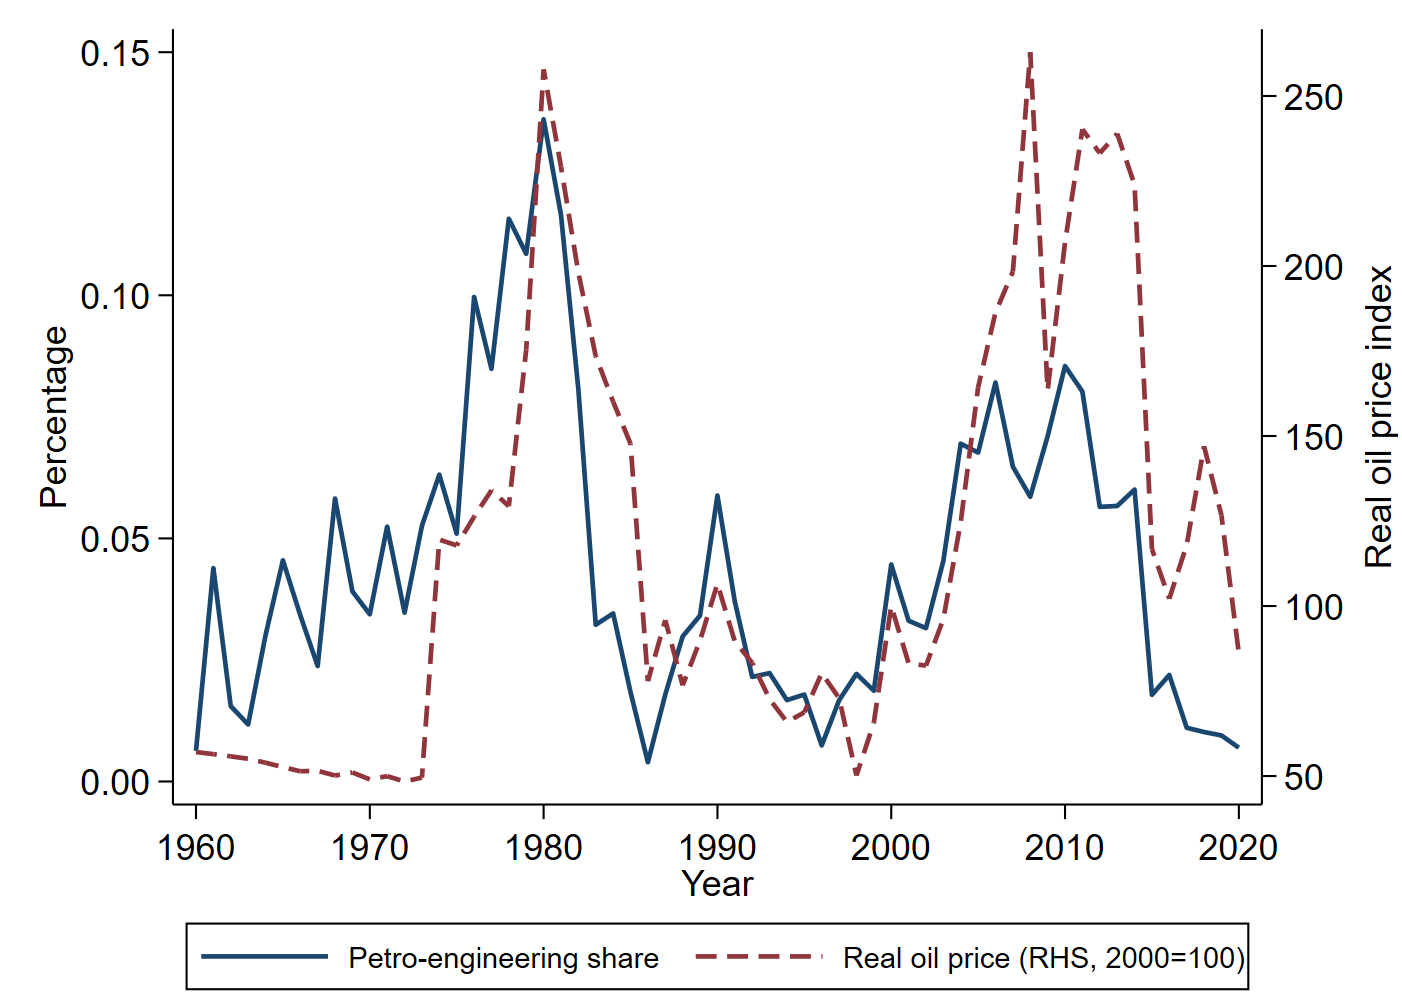
\includegraphics[width=0.99\textwidth]{petro_major_new.png}
  \caption{\textbf{Real oil prices and petroleum engineering enrollment share.} The figure plots the petroleum engineering major share among cohorts born in Texas, North Dakota, and New Mexico (left axis) against the annual real oil price (2000=100, right axis). Cohorts are indexed by the year individuals turned age 18.}
  \label{fig:oil}
\end{figure}









%\begin{proposition}[Capital Underinvestment (Hold-Up Problem)]
%\label{prop:capital}
%This inefficiency is independent of the Hosios condition. For any $\beta_i > 0$, the firm faces a ``hold up" by the worker and cannot capture the full marginal product of its investment. This leads to systematic underinvestment in capital ($k_i^{DE} < k_i^{SP}$).
%\end{proposition}


\subsection{Inefficiency when Hosios condition fails}



\subsubsection{The empirically relevant case: $\eta > \beta$}

The preceding subsection focused on the Hosios benchmark $\beta=\eta$, under which the decentralized equilibrium internalizes the standard search externality. Empirically, however, a relevant case is that workers' bargaining power $\beta$ is lower than the matching elasticity $\eta$,
%empirical evidence suggests a particular direction of departure is most relevant: workers' social contribution to matching exceeds their private bargaining share, 
that is, $\eta > \beta$.

%\paragraph{Empirical evidence:}
The matching elasticity with respect to unemployment, $\eta$, is relatively well identified. \cite{petrongolo2001looking} survey the empirical literature and report estimates typically in the range of  0.5 to 0.7. More recent studies, such as \citep{borowczyk2013match}, are broadly consistent with this range. In contrast, estimates of workers' bargaining power, $\beta$, are more dispersed but generally suggest values below $\eta$. \cite{hagedorn2008cyclical} estimate $\beta \approx 0.05$ in their baseline specification, though this rises to about 0.46 when capital is incorporated into the model. \cite{flinn2006minimum} estimates bargaining power in the range of 0.3-0.4. More recent evidence points to a secular decline in workers' bargaining power: \cite{azar2022labor} document falling labor shares and attribute this partly to declining worker bargaining power, consistent with lower unionization and greater labor market concentration.

%Importantly, sector-specific estimates of $\eta$ and $\beta$ are rare. The available evidence suggests matching-technology parameters are broadly similar across industries \citep{petrongolo2001looking}. Because most empirical studies estimate these parameters at the aggregate level, we maintain the assumption $\eta_m = \eta_s = \eta > \beta_m = \beta_s = \beta$ throughout our analysis, with common values applying to both manufacturing and services.

%\paragraph{Policy relevance:}
%The case $\eta > \beta$ is particularly relevant for industrial policy. When workers under-capture their social contribution to match formation, they face insufficient incentives to enter sectors with high search frictions. This problem is compounded in capital-intensive sectors where the holdup problem simultaneously depresses wages. The interaction between these two distortions creates an especially severe misallocation, as the following proposition demonstrates.





\begin{proposition}[]
\label{prop:double_penalty}
When $\eta > \beta$ and $\epsilon_m>\epsilon_s$, the decentralized equilibrium is inefficient even if the capital is fixed exogenously  at the social planner's level, $k_i = k_i^{SP}$.
\end{proposition}


%From above, the allocation wedge in sector $i$ is:
%\[
%W_i = H_i(\beta_i) - H_i(\eta_i) = \left(\frac{\beta_i}{1-\beta_i} - \frac{\eta_i}{1-\eta_i}\right) P_k k_i (r+s_i) \theta_i.
%\]
%When $\eta_i > \beta_i$, we have $W_i < 0$ for both sectors. The holdup problem (Proposition \ref{prop:capital}) implies $k_i^{DE} < k_i^{SP}$, with the investment shortfall proportional to capital intensity $\zeta_i$. Since the wedge magnitude $|W_i|$ scales with $P_k k_i \theta_i$, which is larger in the more capital-intensive sector, we have $|W_m| > |W_s|$ when $\zeta_m > \zeta_s$. Therefore, $W_m - W_s < 0$, implying $L_m^{DE} < L_m^{SP}$ (Proposition \ref{prop:allocation}(c)).

The gap  between the tightness conditions in the decentralized equilibrium, equation\eqref{eq:DE_char_theta_main},  and in the social planner's allocation, equation \eqref{eq:SPP_theta_condition_boxed},  reflects the familiar inefficiency that arises when Hosios condition fails.

What is new in our two-sector environment is an additional wedge in workers' sectoral choices.  %Compare  sectoral choice conditions \eqref{eq:DE_char_edu_main} and \eqref{eq:SPP_Ls_condition_boxed}.
Substitute the planner's tightness condition \eqref{eq:SPP_theta_condition_boxed} into \eqref{eq:SPP_Ls_condition_boxed} and the decentralized equilibrium's tightness condition \eqref{eq:DE_char_theta_main} into \eqref{eq:DE_char_edu_main}, we have
\begin{align}
    r(\epsilon_m-\epsilon_s) &= \frac{\eta}{1-\eta}[\theta_mP_kk_m(r+s_m)-\theta_sP_kk_s(r+s_s)],   \label{rc_sp}\\
        r(\epsilon_m-\epsilon_s) &= \frac{\beta}{1-\beta}[\theta_mP_kk_m(r+s_m)-\theta_sP_kk_s(r+s_s)].  \label{rc_de} 
\end{align}

Even holding $\theta_i$ and $k_i$ fixed, it is immediate that  when $\eta>\beta$ and $\epsilon_m>\epsilon_s$,  the right-hand side of \eqref{rc_sp} exceeds that of \eqref{rc_de}. Intuitively, the right hand side of \eqref{rc_de}  represents the flow surplus gained by an unemployed worker who enters manufacturing rather than services.  The term $P_kk_i(r+s_i)$ is the user cost of firm investment, and multiplying  by  $\theta_i$ scales this cost by the number of vacancies per unemployed worker. Finally, the factor  $\frac{\beta}{1-\beta}$ converts the firm's flow surplus into worker's surplus via Nash bargaining. 


Because $\epsilon_m>\epsilon_s$, a worker must obtain more surplus in manufacturing than in services to compensate for the higher educational cost. When $\beta<\eta$, the decentralized equilibrium understates the social return to shifting workers toward manufacturing.

%When the bargaining weight $\beta$ rises towards $\eta$, workers capture a larger share of the surplus generated in each sector. Since $m$ sector generates higher surplus than $s$ sector to begin with,  a larger worker share disproportionally increases the attractiveness of $m$ sector more than $s$ sector. 



\begin{proposition} \label{prop:small_beta}
Under $\beta<\eta$, the social planner's allocation can be implemented using three policy instruments $\{\tau^{K**}_i, \tau^{T**}_i, \tau^{L**}_i\}$: a sector-specific investment subsidy, a sector-specific lump-sum tax on firms, and a training subsidy for manufacturing workers. Specifically, 


    
\begin{align}
     \tau^{K**}_i &= 1- \frac{(1-\beta)(r+s_i+q_i)}{r+s_i+(1-\beta)q_i} >0,\\
  \tau^{T**}_i      &=  \frac{q_i(1-\eta)}{(r+s_i)}\Phi_i - \tau^{K**}_iP_kk_i/P - \frac{q_i(1-\beta)[p_if_i(k_i)/P-z]}{(r+s_i)D_i(\beta)},  \\
   \tau^{L**}_m & =   r(\epsilon_m-\epsilon_s) -  [\theta_m q_m \,\eta\, \Phi_m-  \theta_s q_s\,\eta\, \Phi_s]  \\
   & \quad - [ \theta_mq_m\beta \frac{p_mf_m(k_m)/P-z}{D_m(\beta)}   
   -\theta_sq_s\beta \frac{p_sf_s(k_s)/P-z}{D_s(\beta)}],\\
      \tau^{L**}_s&=0,
\end{align}

where    $\{\theta_i, k_i, q_i, L_i\} = \{\theta_i^{SP}, k_i^{SP}, q_i^{SP}, L_i^{SP}\}$,  and

\begin{align*}
    D_i(\beta)&= r+s_i+(1-\beta)q_i+\beta\theta_iq_i, \\
    \Phi_i & = \frac{p_if_i(k_i)/P-z}{D_i(\eta)}.
\end{align*}


\end{proposition}


% % ===============================================================
% \subsection{Policy for First–Best Implementation}
% \label{sec:policy_firstbest}
% % ===============================================================

% To restore efficiency, we introduce two instruments: a targeted subsidy to STEM entrants 
% and a two–part capital policy. The government finances these policies with a lump–sum 
% tax, ensuring a balanced budget in steady state.

% \paragraph{STEM education subsidy:} 
% Each STEM entrant receives a lump–sum subsidy 
% $\gamma^\star = r\,\Delta^{\text{Edu}}$, chosen to close the education wedge 
% (derivation in Appendix~C).


% \begin{equation}\label{eqn:gamma}
%     \gamma^* = r\,\Delta^{\text{Edu}} = r[  \frac{p_mA_m\phi_m(k_m)}{D_m(\theta_m)}
% -\frac{p_sA_s\phi_s(k_s)}{D_s(\theta_s)}  ]
% \end{equation}

% \paragraph{Capital instruments.}
% Firms under--invest in $k_i$ because they retain only a $(1-\beta)$ share of the match 
% surplus. To correct this, introduce:
% \begin{enumerate}[leftmargin=1.5em]
% \item a \emph{capital tax credit} $\tau_i^K$ that lowers the user cost of capital to 
% $(1-\tau_i^K)\tilde r_i$,
% \item a \emph{license fee} $\psi_i$ per job position (vacant or filled) to preserve free 
% entry.
% \end{enumerate}
% The values that implement the planner’s allocation are
% \begin{equation}\label{eqn:tauk}
% \tau_i^{K\star}(\theta_i)
% = 1-\frac{1+\tfrac{s_i}{q_i(\theta_i)}}
% {1+\tfrac{r+s_i}{(1-\beta)\,q_i(\theta_i)}}, 
% \end{equation}
% \begin{equation}\label{eqn:psi}
% \psi_i^\star = \tau_i^{K\star}(\theta_i^{SP})\,\tilde r_i k_i^{SP},
% \end{equation}
% with derivations in Appendix~C.



% \begin{proposition}[First–best implementation]
% Under the Hosios condition, $\beta=\eta_i(\theta_i)$, the policy tuple
% \[
% (\gamma,\;\tau_m^K,\;\tau_s^K,\;\psi_m,\;\psi_s)
% = (r\Delta^{\text{Edu}},\;\tau_m^{K\star},\;\tau_s^{K\star},\;\psi_m^\star,\;\psi_s^\star)
% \]
% implements the planner’s allocation:
% \[
% (\theta_i^{DE},k_i^{DE},L_s^{DE})=(\theta_i^{SP},k_i^{SP},L_s^{SP}),
% \qquad i\in\{m,s\}.
% \]
% \end{proposition}

% \paragraph{Budget balance:}
% At $(\tau_i^{K\star},\psi_i^\star)$, the tax credit and license fee offset, leaving only 
% the STEM subsidy as a net fiscal cost:
% \[
% T^\star = r\,\Delta^{\text{Edu}}\,L_m^{SP}.
% \]
% This can be financed with a lump–sum tax on households and/or firms.

% \paragraph{Welfare equivalence:}
% Since decentralized FOCs match the planner’s, allocations coincide. By distributing 
% the lump–sum tax appropriately across households and firms, individual payoffs also 
% match the planner’s.
\section{Calibration}\label{section calibration}
\color{black}

We calibrate the benchmark model at an annual frequency to Chile.  Several parameters are set exogenously based on direct empirical counterparts or standard values in the literature. While we target Chilean moments whenever possible, for some parameters we rely on  U.S. evidence because of  data limitations. 

%We set the CES parameter $\rho=-1$, implying an elasticity of substitution between industrial and service goods of $\epsilon=\tfrac{1}{1-\rho}=0.5$. Evidence generally supports an elasticity below unity, making $m$ and $s$ complements (e.g., \citealp{boppart2014structural}; see also \citealp{ngai2008trends} for lower estimates). For job-specific capital, we use $\phi(k_i)=k_i^{\zeta_i}$. Using BLS labor–compensation data (2010–19), capital income shares are $0.74$ in manufacturing and $0.31$ in nonfarm business excluding manufacturing, so we set $\zeta_m=0.74$ and $\zeta_s=0.31$.


We set the elasticity of substitution between  domestic  and foreign services $\nu=2$,  within the range commonly used in applied trade models, for example, in \cite{GTAP}. This implies that domestic and  foreign  services are gross substitutes. We normalize the foreign prices $p_m$ and $p_s^F$ to one. We set the total labor force to one and choose the sum of manufacturing and service labor forces $L=0.94$, so that the implied agricultural labor force -- treated as exogenous -- is 6 percent of the total labor force. This targets Chile's observed agricultural employment share, which is about 6\% in 2024.   We assume the production functions are in Cobb-Douglas form:  $f_i(k_i)=A_ik_i^{\xi_i}$. We normalize the service sector productivity  $A_s$ to one. We set  $\xi_m$ and $\xi_s$, to be 0.65 and 0.3, respectively. These values are consistent with the evidence that capital’s income share  is substantially higher in industry than in services (0.63 vs. 0.34 in 2022, based on Comisión Nacional de Productividad (CNEP) data). Because sectoral factor-income shares are measured with error, we treat these numbers as informative benchmarks  rather than exact targets.


For labor market parameters, we normalize the  matching efficiency to one, following standard practice (\citealt{mortensen1994job, petrongolo2001looking}).  We set the elasticity of the matches with respect to unemployment to $\eta = 0.5$, the midpoint of the empirical estimates surveyed by \citet{petrongolo2001looking}, and in line with standard calibrations (e.g., \citealt{hallmilgrom2008, menzio2016directed}).  In the benchmark calibration, we set  workers' bargaining power to $\beta=\eta$, so that the standard matching externality is shut down. We will report the results for the case $\beta<\eta$.  
 %We set home production $z=1$. In equilibrium, $P_sz$ is about $30$ percent of the wage income, which is broadly in line with the range in the literature. 

%Consistent with \citet{shimer2005cyclical}, we also set workers’ bargaining weight equal to this elasticity. For the service sector separation rate, we adopt $s_s=0.20$ annually. This value lies between the lower bound of about 13\% annually implied by \citet{fernandez2010}, and the upper bound of 34\% annually reported in \citet{shimer2005cyclical}, and is further supported by JOLTS industry data showing annual separations of 20–27\% in service subsectors such as finance, education, and health \citet{blsJOLTS}.




%Finally, we calibrate an exogenous retirement parameter $\chi$ to capture demographic exits from the labor force. We set $\chi=0.025$, corresponding to an expected working life of 40 years. Retirements are offset by an equal inflow of new entrants, so that the labor force remains stationary. Retirement is distinct from $s_i$: while $s_i$ governs job turnover (employment–unemployment flows), $\chi$ matters only for fiscal calculations such as the annualized cost of education subsidies.

\begin{table}[h!]
\centering
\caption{Exogenously Set Parameters:}\label{table_set_parameters}
%\begin{adjustbox}{width=0.8\columnwidth,center}
\begin{tabular}{||c c c c||}\hline
\textbf{Parameter} & \textbf{Description} & \textbf{Value} & \textbf{Source} \\\hline\hline
$\nu$ & CES aggregator coefficient & $2$ & \cite{GTAP} \\
$m$ & Matching efficiency & $1$ & Normalization \\
$\eta$ & Matching elasticity & $0.5$ & \cite{petrongolo2001looking} \\
$\beta$ & Worker bargaining weight & $0.5$ & Hosios condition \\ %\cite{shimer2005cyclical} \\
%$s_s$ & Service separation rate (annual) & $0.20$ & BLS/JOLTS \\
%$A_m$ & Manufacturing technology & $1$ & Normalization \\
$A_s$ & Services technology & $1$ & Normalization \\
$p_m$ & $m$ goods price & $1$  & Normalization  \\
$p_s^F$ & Foreign service goods price & 1 & Normalization \\
$L$  & sum of $L_m$ and $L_s$  & 0.94  &  Agriculture labor force $\sim$ 0.06\\
$\zeta_m$ & Capital share in manufacturing & $0.65$ & CNEP \\
$\zeta_s$ & Capital share in services & $0.3$ &  CNEP
%$\chi$ & Retirement (annual rate) & $0.025$ & 40-year working life 
\\\hline
\end{tabular}
%\end{adjustbox}
\end{table}

\paragraph{Endogenously calibrated parameters. } The remaining parameters are calibrated to match moments in the decentralized equilibrium.  Their values are reported in Table \ref{table_calibrated_parameters}. We choose the  preference weight on manufacturing goods, $\alpha$,  so that $L_m=21.7\%$ in equilibrium, matching Chile's industrial employment share in 2024. The separation rates, $s_m$ and $s_s$, are pinned down by  sectoral unemployment rates.  Specifically, we target a 6.9\% unemployment rate  in each sector, which equal to the average unemployment rate in Chile during 2015-19.\footnote{\cite{CNEP2024STEM} documents that unemployment rates for workers who chose STEM majors are similar to those in non-STEM tracks. } %Although this value is lower than the separation rates typically used in the search-model literature (e.g., \cite{shimer2005cyclical}), it ensures consistency with the observed unemployment differential across sectors. 
The time discount rate $r$ is pinned down by the aggregate capital-to-output ratio $\frac{P_kK}{Y^N}$. In the model, total capital is  $K\equiv \sum_i k_i(n_i+v_i)$, and nominal output $Y^N\equiv p_mY_m+p_sY_s$.    We set $r$ to 0.06, which implies a capital-to-output ratio $K/Y^N = 2.9$. This matches Chile's  non-mining, non-agriculture capital-to-output ratio in 2022 (2.9).\footnote{Chile’s mining sector is capital intensive and accounts for about 10–12 percent of aggregate output. We therefore target the capital-to-output ratio excluding mining to be more representative of other small open economies. Including mining, Chile’s aggregate capital-to-output ratio is about 3.3 in 2022.} and is  also consistent with the range of estimates in \cite{feenstra2015next} for a broader set of countries.\footnote{See Appendix C in \cite{feenstra2015next}.}

We calibrate the relative productivity, $A_m/A_s$, to match the sectoral wage ratio $w_m/w_s$, which \cite{elvery2021manufacturing} estimate to be 4-14 percent for the United States.  Finally, we calibrate the educational cost differential, $\epsilon_m-\epsilon_s$, to $70$ percent of $w_m$ based on \cite{altonji2018costs}, who  document training cost by major. Using their estimates, we compare the average training costs in STEM and non-STEM fields, %and compare the difference in training costs with per worker income (calculated from disposable income and employment-to-population ratio) from U.S. Bureau of Economic Analysis. 
and obtain a difference  equivalent to 70-75 percent of the per worker income.  The parameter $\chi$ governs the equilibrium service import-to-GDP ratio. Because of the balanced trade assumption, the closest data counterpart is goods trade surplus-to-GDP ratio. 
We choose $1-\chi=0.0044$ so that the goods trade surplus is about 5.5 percent of GDP , matching Chile's average trade surplus in 2023-24.  Finally, we set unemployment income to $z=2.5$ which implies a  home production-to-wage ratio of 0.30 in equilibrium, within the range  of 0.25-0.35 estimated by \cite{house2008valuing}.

\begin{table}[h!]
\centering
%\footnotesize
\caption{Internally Calibrated Parameters.}\label{table_calibrated_parameters}
%\begin{adjustbox}{width=0.95\columnwidth,center}
\begin{tabular}{||c c c c||}\hline
\textbf{Parameter} & \textbf{Description} & \textbf{Value} & Data Moment \\\hline\hline
$\alpha$ & Preference weight on $m$ goods & $0.174$ & Industrial employment share \\
$s_m$ & Separation rate in $m$ & $0.048$ & Unemployment rate in $m$  \\
$s_s$ & Separation rate in $s$ & $0.115$ & Unemployment rate in $s$ \\
$r$ & Discount rate (annual) & $0.06$ & Capital-output ratio \\
$1-\chi$ & Service import weight & 0.0044 & Goods trade balance-to-GDP \\
$A_m/A_s$   & relative productivity & 2.0  &   sectoral wage ratio\\
$\epsilon_m-\epsilon_s$ & Education cost differential & 6.0 &  $\Delta$ training cost-to-labor income \\ 
$z$  & Home production utility  & 2.5 & Home production-to-wage
\\\hline
\end{tabular}
%\end{adjustbox}
\end{table}

\noindent
%Finally, we choose the discount rate $r$ so that the equilibrium capital-to-output ratio matches with the data. We set $K/Y$ target at 2.5, consistent with the range in \cite{feenstra2015next} and \cite{caselli2007marginal}. This yields a discount rate $r=0.085$. We also report untargeted moments: 




\begin{table}[h!]
\centering
%\footnotesize
\caption{Matching the calibration targets and non-targeted moments.}\label{table_calibration_targets}
%\begin{adjustbox}{width=0.7\columnwidth,center}
\begin{tabular}{||c c c||}\hline
\textbf{Moment} & \textbf{Target} & \textbf{Model} \\\hline\hline
Share of industrial labor, $L_m$ & $ 21.7\%$ & 21.7\% \\
Unemployment rate ($m$)  & $ 6.9\%$ & $6.9\%$ \\
Unemployment rate ($s$)  & $ 6.9\%$ & $6.9\%$ \\
Capital-to-output ratio & $ 2.9$ & $2.9$ \\
%Labor income share ($m$)  & $0.36$ & $0.39$ \\
%Labor income share ($s$)  & $0.66$ & $0.75$ \\
Goods trade surplus-to-GDP & $5.4\%$ &  $5.4\%$ \\
Wage ratio $w_m/w_s$ & $1.09$ & $1.09$  \\
Training cost differential-to-wage & $0.72$ & 0.71 \\
Home production-to-wage     &  $0.30$   &   0.29  \\
% & & \\  
%\textbf{Non-Targeted Moments} & & \\
%Capital formation-to-GDP & $0.23$ & $0.225$ 
%Aggregate unemployment rate & $0.06$–$0.10$ & $0.08$ 
\hline
\end{tabular}
%\end{adjustbox}
\end{table}

\section{Quantitative Results}\label{section results} 

\subsection{Decentralized equilibrium versus social planner.}
Table \ref{DE_SP} compares the decentralized equilibrium (DE) with the social planner's allocation (SP). Relative to the dentralized equilibrium, the planner chooses a higher capital–output ratio, $K/Y=3.3$ instead of  $2.9$. This reflects the holdup inefficiency in the decentralized economy: because wages are bargained after capital is sunk, firms internalize only a fraction of the marginal match surplus when choosing vacancy capital, which leads to underinvestment. 

%In the DE, capital is under-provided because of the hold-up wedge in wage bargaining. A social planner would like to choose higher capital levels in both sectors.   %The planner raises $k_m$ and $k_s$ (to $334$ and $53$ from $279$ and $40$), which lifts relative labor productivity $f_m(k_m)/f_s(k_s)$ (from $19.4$ to $19.9$). with a particularly pronounced rise in manufacturing sector due to its greater capital intensity.
%The planner raises $k_m$ by $19.6$ percent, lower than $k_s$ ($31.4$ percent). However,  
Capital deepening raises output per worker in both sectors, with a larger increase in manufacturing because production there is more capital intensive.  Relative to the decentralized equilibrium, real labor productivity, $f_m(k_m)$,  is 13.7 percent higher, compared with 10.0 percent in services. Total output also rises more in  manufacturing  than services, by 17.9 percent versus 7.4 percent. 






The social planner also  chooses a higher industrial labor force share than the DE: $L_m$ rises by $1.0$ percentage point.  Intuitively, because manufacturing is more capital intensive, correcting the holdup wedge raises match surplus in manufacturing more than in services. This increases the marginal gain from  rellocating one more worker from services to manufacturing. The open-economy goods block dampens the relative-price adjustment, so the reallocation primarily through labor quantities rather than relative prices. 

%This is because under planner's allocation, capital deepening implies that real labor productivity rises more in manufacturing sector than services, while the relative prices $p_s/p_m$ is relatively stable due to the open economy feature and the higher domestic manufacturing goods demand for higher capital consumption. Therefore, the nominal labor productivity in manufacturing rises more than services under the planner's allocation than decentralized equilibrium, incentivizing more job creation in the manufacturing sector.  


Unemployment rates are \textbf{higher under the social planner} in both sectors. Intuitively, the planner chooses higher capital per worker, $k_i$, than in the decentralized equilibrium.  Because vacancy creation requires installing job-specific capital, a higher $k_i$ raises the cost of vacancy creation.  The planner hence chooses lower market tightness,  $\theta_i^{SP}< \theta_i^{DE}$, which reduces job-finding rates and increases unemployment rates. Finally, real output is about 11.3\% higher in planner's allocation, driven almost entirely driven by capital deepening and the resulting increase in labor productivity. %Relative prices hardly move ($p_m/p_s\approx0.47$ in both). 

%Two opposing forces drive this outcome.  
%First,  capital deepening under the SP allocation 
%boosts the productivity sector of $m$.  Because $m$ and $s$ are complements,  the social planner would like  to choose a lower level of labor input than in the DE.  Second, the  industrial sector's labor market suffers from a more severe holdup problem. Absent  the capital deepening effect on relative productivity -- i.e., holding capital level fixed -- the industrial sector's employment in the DE is inefficiently low, as  first noted by \cite{navarro2011efficiency}.  Table \ref{DE_SP_exogenous_k} illustrates this point by computing the SP allocation when capital levels $k_i$ of both sectors, the social planner chooses a higher $L_m$, reflecting the inefficiently low industrial employment that solely stems from labor market frictions. 

%When both forces operate -- endogenous capital choices and labor market frictions -- our baseline parameters imply that the first effect, capital deepening, dominates, so industrial employment is ultimately lower in the SP allocation. 



\begin{table}[H]
 \caption{DE and SP  Allocation under Endogenous Capital Level} \label{DE_SP}
\centering
%\begin{adjustbox}{width=0.6\columnwidth,center}

 \begin{tabular}{||c c c c||} 
 \hline
 \textbf{Moments} & \textbf{DE} & \textbf{SP}  & $\Delta$ \\  
 \hline\hline
  Labor force share ($m$), $L_m$ & 21.7\%  & 22.7\% & +1.0  pp \\
  Employment share ($m$), $n_m/(n+L_a)$ & 21.6\% & 22.7\%  & +1.1 pp \\
%   Employment ($m$), $(L_m-u_m)/L$ &  21.6\%  & 22.7\% & +1.1 pp  \\
%   Employment ($s$), $(L_s-u_s)/L$ &  66.0\%  & 64.5\% & -1.6 pp  \\
  Unemployment rate ($m$), $u_m/L_m$ & 6.9\% & 7.5\% & +0.6 pp  \\ 
   Unemployment rate ($s$),  $u_s/L_s$ & 6.9\% & 7.9\% & +1.0 pp \\ 
    Tightness, $\theta_m$ & 0.42 & 0.35  & $-0.07$ \\
  Tightness, $\theta_s$ & 2.40 & 1.77  & $-0.63$ \\
   Capital per worker ($m$), $k_m$ & 841 &  1024  & $ +21.8\%$ \\ 
      Capital per worker ($s$), $k_s$ & 84 &  116  & $ +37.5\%$ \\ 
  Capital-to-output ratio, $K/Y$ & 2.9 & 3.3    &   $+0.4$\\
  Total capital,  $K$  & 242  & 309 & $ + 27.5\% $\\
  Relative prices, $p_s/p_m$ & 20.1  &  20.1  &  $-0.1\%$ \\
  Real labor productivity, $f_m(k_m)$ & 79.6 & 90.5 & $+13.7\% $\\ 
Real labor productivity, $f_s(k_s)$ & 3.8 & 4.2 & $+10.0\% $\\ 
Output ($m$), $Y_m$  & 32.2 & 38.0 & $+17.9\%$ \\
Output ($s$), $Y_s$  & 2.5 & 2.7 & $+7.4\%$ \\
%  \textbf{Non-Targeted Moments} &  &  \\
% Relative wages, $w_m/w_s$ &  1.09 & 1.08 \\
% Relative output, $Y_m/Y_s$ & 13.6  & 14.9  & $+ 1.3$\\
 Real output, $Y$ &  11.8   &  13.1 & $+11.5\%$ \\
 % Training Expenses/GDP & 0.75\% & 0.75\% \\ 
 [1ex] 
 \hline
 \end{tabular}
%\end{adjustbox}
 
\end{table} 





\subsection{Policy when $\beta=\eta$}

\subsubsection{Policies that implement the planner's allocation.} Under $\beta=\eta$, the decentralized equilibrium is inefficient only because vacancy capital is sunk before bargaining, which generates the holdup wedge.  Proposition \ref{prop_implementation_hosios} shows that the planner's allocation can be implemented by a subsidy $\tau^{K*}_i$ on newly created vacancies, together with an offsetting lump sum tax $\tau^{T*_i}$ that preserves the free entry condition. Under the baseline calibration,  this yields $\tau^{K*}_m = 5.6\% $ and $\tau_s^{K*}= 15.7\%$. 
%Note that the investment subsidy is a one-time subsidy for each newly created vacancy. 
Because the subsidy $\tau^{K*}_i$ applies the flow of newly created vacancies, the  
aggregate fiscal cost of the investment subsidy measured in units of final consumption unit, is

\begin{align}
\mathrm{Sub}_K \;=\; \sum_i \tau^{K*}_i \frac{P_k\,k_i\,x_i}{P} \;=\; \sum_i \tau^{K*}_i \frac{P_k\,k_i\,s_i\,(n_i+v_i)}{P}.
\end{align}

where the second equality uses the steady-state condition $x_i = s_i(n_i+v_i)$. 
Under the baseline calibration, this subsidy a 2.4\% of GDP per year. It is fully financed by the lump sum tax $\tau^{T*}$. 

%The higher subsidy rate in services than manufacturing reflects the differences in sectoral separation rates and vacancy filling rates. 
%is mainly because the services sector has a much lower per capita capital, hence in percentage terms the subsidy rate in services sector is higher than manufacturing. 

%This investment subsidy, as explained in Proposition \ref{prop_implementation_hosios}, is fully financed by the lump-sum tax $\tau^T_i$. 

\subsubsection{Investment subsidy  only.}

In practice, the  government may not be able to levy employment-based lump sum taxes due to political constraints, and sector-specific investment subsidies may be difficult to administer. %We therefore consider a restricted policy that sets  $\tau^K_m=\tau^K_s= \tau^{K*}_m$ and $\tau^T_m=\tau^T_s=0$. 
Table \ref{policytable} therefore reports equilibrium outcomes under three policy configurations.  DE1 implements the planner's allocation. DE2 sets $\tau^{T}=0$ while keeping sector-specific investment subsidies. DE3 imposes a sectoral uniform subsidy and again set $\tau^T_i=0$.


\paragraph{Labor market outcomes.} Removing the lump-sum tax in DE2 and DE3 induces over-entry. Market tightness, $\theta_i$, rises in both sectors, and vacancy-filling rates, $q_i$, fall. The higher tightness increases job-finding rates and lowers unemployment. The industrial labor force share rises further in DE2 relative to DE1, reflecting stronger vacancy creation in manufacturing when  the lump sum tax is absent. 

\paragraph{Capital, output, and welfare.} Relative to DE1, DE2 and DE3 feature  slightly lower capital-to-output ratios. Intuitively, when lump sum tax is absent, firms have stronger incentives to create vacancies than to deepen capital. Output differences are modest: $Y_m$ is slightly higher in DE2 while $Y_s$ is slightly lower. %Real consumption is essentially the same across two policies: higher $Y_m$ in DE2 is offset by lower $Y_s$ and higher investment absorption.
Welfare in DE2 slightly lower than that in DE1 because the lower unemployment  also means less home production.

\paragraph{Fiscal cost.} DE1 is fiscally neutral, whereas DE2 and DE3 require net fiscal costs of 2.4 and 2.1 percent of GDP, respectively. 


\begin{table}[H]
 \caption{Equilibrium Allocations under Taxes and Subsidies when $\beta=\eta$} \label{policytable}
\centering
 \begin{tabular}{||c c c c||} 
 \hline
 \textbf{Moment} & \textbf{DE1}  & \textbf{DE2 }  & \textbf{DE3}\\  
 Description    & Implements SP & Only $\tau^K$  & Only uniform $\tau^K$ \\
  $\tau^K_i$  &   $\tau^K_i=\tau^{K*}_i$     &  $\tau^K_i=\tau^{K*}_i$    &  $\tau^K_i = \tau^{K*}_m$  \\
    $\tau^T_i$  &   $\tau^T_i=\tau^{T*}_i$     &  0    &   0  \\
 \hline\hline
  Industrial labor force, $L_m$   & 22.7\%& $23.2\%$&   $22.7\%$ \\
  Industrial unemploy. rate, $u_m/L_m$ & 7.5\%& $6.8\%$&  $6.8\%$  \\ 
   Services unemploy. rate, $u_s/L_s$  & 7.9\%&   $6.8\%$&   $6.8\%$  \\ 
  Capital-to-output ratio, $K/Y$  & 3.3& 3.3  &  3.1\\
  Tightness, $\theta_m$  & 0.35&  0.44&  0.43  \\
    Tightness, $\theta_s$  & 1.77&  2.52&  2.49 \\
 % Vacancy-filling rate, $q_m$ & 1.72 &   1.54   &  1.55 \\
 %   Vacancy-filling rate, $q_s$  & 0.76 &   0.64   &  0.65 \\
%  Total capital,  $K$  & 252  & 319 & $ + 27\% $\\
 % Relative prices, $p_s/p_m$ & 0.473  &  0.474 \\
%  Labor productivity, $A_m\f_m(k_m)/A_s\f_m(k_s)$ & 42.1 & 43.5 & $+3.3\% $\\ 
%  \textbf{Non-Targeted Moments} &  &  \\
% Relative wages, $w_m/w_s$ &  1.09 & 1.08 \\
 Real output, $Y_m$    & 38.0   & 38.3  & 37.4\\
 Real output, $Y_s$ &   2.7  &  2.7 &  2.64 \\
% Real consumption $C$ & 4.07  & 4.07  & 4.01  \\  
 Welfare, $W$  &     4.18    &  4.15      &  4.09           \\
 Annual fiscal cost ($\%$ of GDP)  &   0   &  2.4  & 2.1 \\
 % Training Expenses/GDP & 0.75\% & 0.75\% \\ 
 \hline
 \end{tabular}
%\end{adjustbox}
 
\end{table} 



\subsection{Optimal taxes and subsidies when $\beta<\eta$.}

We now relax the Hosios condition and consider the empirically relevant case in which workers' bargaining power, $\beta$, is lower than the matching elasticity, $\eta$. We set $\beta=0.3$ while holding all other parameters, including $\eta=0.5$, at their benchmark values. This departure introduces the standard search externality, so that vacancy creation is no longer efficient. It also generates the additional wedge in workers' sectoral choices that is central to our model:  because workers capture too small a share of match surplus,  their sectoral choices remain distorted even after the vacancy-creation externality is corrected.  

To illustrate this point, Table \ref{policytable_small_beta} reports the equilibrium outcomes under three policy settings. First, DE-A is the decentralized equilibrium under $(\beta, \eta)=(0.3, 0.5)$ with no policy instruments. Second, DE-B implements the social planner's allocation using the full policy package: sector-specific investment subsidies and lump sum taxes, $\{\tau^{K**}_i, \tau^{T**}_i\}_{i \in \{m,s\}}$, together with a manufacturing training subsidy   $\tau^{L**}_m$.\footnote{Note that $\tau^{L**}_s=0$ in Proposition \ref{prop:small_beta}.} Third, DE-C applies the same firm-side policies but sets  $\tau_m^{L}$ =0.  This last case isolates the additional sectoral choice wedge: if correcting firm-side distortions were sufficient,  DE-C would coincide with the planner's allocation. 




Relative to the benchmark decentralize equilibrium with $\beta=\eta=0.5$ (column DE), lowering workers' bargaining power to $\beta=0.3$ in DE-A raises firms' incentives to create vacancies, resulting in substantially higher market tightness and lower unemployment  in both sectors. Manufacturing output increases modestly, while service output is changes little. Despite these gains, welfare falls slightly as the labor market becomes excessively tight, allocating too many resources to vacancy creation and reducing the time spent on home production.  %This illustrates the standard inefficiency from violating the Hosios condition. 

The comparison between DE-B and DE-C highlights the additional wedge in sectoral choice. By construction, DE-B coincides with the planner's allocation. In contrast, when the training subsidy is shut down, the labor force share in manufacturing falls sharply in DE-C relative to DE-B. The mechanism is precisely the sectoral wedge implied by $\beta<\eta$: even after firm-side distortions are corrected, workers capture too small a share of surplus to justify the move into manufacturing. A targeted subsidy to manufacturing skill acquisition therefore plays a distinct role in correcting this wedge. 




\begin{table}[h!]
 \caption{Equilibrium allocations, $\beta<\eta$} \label{policytable_small_beta}
\centering
\begin{adjustbox}{width=1\columnwidth,center}
 \begin{tabular}{||c c c c c||} 
 \hline
 \textbf{Moment} &  \textbf{DE} & \textbf{DE-A}  & \textbf{DE-B }  & \textbf{DE-C}\\  
 Description  & Benchmark  & DE ($\beta<\eta$) & Implements SP  &  No training subsidy \\
$\beta$   & 0.5 & 0.3  & 0.3  &  0.3 \\
$\eta$   & 0.5 & 0.5  & 0.5  &  0.5 \\
  $\tau^K_i$ & 0 &    0    &  $\tau^K_i=\tau^{K**}_i$    &  $\tau^K_i = \tau^{K**}_i$  \\
    $\tau^T_i$ & 0 &  0    &  $\tau^T_i=\tau^{T**}_i$   &   $\tau^T_i=\tau^{T**}_i$  \\ 
        $\tau^L_m$ & 0 &  0    &  $\tau^L_m=\tau^{L**}_m$    &   0  \\ 
 \hline\hline
  Industry labor force, $L_m$ & 21.7\%& 21.9\%& $22.7\%$&   $20.3\%$\\
  Industry unemp. rate, $u_m/L_m$ & 6.9\%& 4.6\%& $7.5\%$&  $7.1\%$\\ 
   Services unemp. rate, $u_s/L_s$ & 6.9\%& 4.8\%&   $7.9\%$&   $8.4\%$\\ 
  Capital-to-output ratio, $K/Y$ & 2.9& 3.0    & 3.3&  3.3\\
  Tightness, $\theta_m$ & 0.42& 0.98&  0.35&  0.40\\
    Tightness, $\theta_s$ & 2.40& 5.76&  1.77&  1.59\\
  %Vacancy-filling rate, $q_m$ & 1.72 &   1.54   &  1.55 \\
  %  Vacancy-filling rate, $q_s$  & 0.76 &   0.64   &  0.65 \\
%  Total capital,  $K$  & 252  & 319 & $ + 27\% $\\
 % Relative prices, $p_s/p_m$ & 0.473  &  0.474 \\
%  Labor productivity, $A_m\f_m(k_m)/A_s\f_m(k_s)$ & 42.1 & 43.5 & $+3.3\% $\\ 
%  \textbf{Non-Targeted Moments} &  &  \\
% Relative wages, $w_m/w_s$ &  1.09 & 1.08 \\
 Real output, $Y_m$ & 32.2& 32.7& 38.0& 33.8\\
Real output, $Y_s$ & 2.5 & 2.6  &  2.7 &  2.7 \\
 Real consumption $C$   & 3.8& 3.8& 4.1& 3.9\\  
 Welfare, $W$  &   3.9& 3.8&  4.2&  4.0\\
 %Annual fiscal cost ($\%$ of GDP)  &   0   &  2.3  & 2.1 \\
 % Training Expenses/GDP & 0.75\% & 0.75\% \\ 
 \hline
 \end{tabular}
%\end{adjustbox}

 \end{adjustbox}
\end{table} 




\subsection{Trade openness and sectoral employment}


In our model, greater service trade openness, captured by a higher value of $1-\chi$,  raises the demand for imported services. Under balanced trade, higher service imports require higher manufacturing exports, which raises labor demand in manufacturing and shifts workers towards that sector.   This mechanism is present even in a frictionless small open economy. 

Search frictions, however, affect the adjustment margin. As service trade openness rises, imported services account for a larger share of the service consumption basket. Because imported services price is cheaper than domestically produced services, service price index $P_s$ falls. This lowers the relative prices of final consumption compared with both manufacturing and services, $P/p_m$  and $P/p_s$. and reduces the value of home production $z$ relative to wages in both sectors and thereby lowering equilibrium unemployment. 

To illustrate the impact of greater service trade openness, we increase the service-import weight in the service basket from $1-\chi$ to $1-\chi'$,  where $1-\chi' = 3(1-\chi)$. Several changes to the equilibrium follow. First, the service import-to-GDP ratio increases from 5.4 percent to 14.0 percent. Second, because trade is balanced, manufacturing exports also rise, raising  manufacturing labor force share from 22.7 percent to 28.9 percent. Third, unemployment rates in both decline, reducing aggregate unemployment rate declines from 6.9 percent to 6.7 percent. This decline is largely driven by the decline of service price $P_s$ and final good consumption $P$ relative to $p_m$, which reduces the value of home production relative to wages. 

%As shown in Figure \ref{fig:Lm_u_Xm},  lower unemployment attenuates the reallocation of labor across sectors. 

%attenuate this reallocation of labor force: unemployment falls as as openness increases, compared to a frictionless model benchmark. Lower unemployment, in turn, dampens the needed sectoral reallocation of labor force: the increase in $L_m$ is milder when there are search frictions. 
%The intuition why unemployment declines is that increased openness lowers the price of service composite $P_s$, which reduces the value of home production for unemployed workers.
%\footnote{A related mechanism appears in the literature on the rise of female labor supply: cheaper household appliances reduced the value of home production relative to formal jobs and and encouraged female labor participation. } As a result, the labor search frictions are mitigated and unemployment rates are lower when openness increases, as shown in Figure \ref{fig:Lm_u_Xm}. 






\section{Conclusion}\label{section conclusion}

This paper studies the chicken-and-egg problem in manufacturing development: should policy prioritize boosting investment or closing sector-specific skill gaps? We develop a two-sector small open economy model with DMP-style search and matching frictions address this question.  Our key mechanism is job-specifc  capital chosen before wage bargaining, which creates a capital holdup distortion. 
The policy implication depends on the Hosios condition. When the Hosios condition holds, correcting capital underinvestment alone is sufficient to replicate the planner's allocation. The optimal policy consists of an investment subsidy, fully financed by lump sum tax on firms. When the Hosios condition fails, an additional wedge distorts workers' sectoral choices beyond the standard search externality, implying a role for targeted training subsidies alongside investment incentives.

%Our framework demonstrates that \textit{labor misallocation across sectors} is a critical margin in structural transformation failures. When capital holdup and search frictions interact, manufacturing development requires coordinating firm investment and worker skill acquisition. Policies targeting only one margin systematically undershoot efficiency, with the optimal mix depending on how match surplus is divided. This coordination mechanism is consistent with \cite{han2020industry}, who document that 1980s oil price increases triggered higher enrollment in petroleum-related majors, confirming that educational choices respond endogenously to sectoral labor demand.

% A key premise is the shift in labor demand  affect educational choices. This premise is consistent with the evidence in \cite{han2020industry}, who documents that the increase in oil prices was followed by increased enrollment in petroleum related college majors in the 1980s. 

\newpage
\startappendix
























\newpage
% ===============================================================
\appsection{Decentralized equilibrium with policy instruments}\label{appendix:DE_policy}

% ===============================================================

This appendix derives the decentralized equilibrium (DE) with policy instruments: $\tau_i^K$ for investment subsidy, $\tau^L$ for education, and..   . Starting from the Bellman equations:

\begin{align}
rJ_i^U &= \theta_i q_i(\theta_i)\big(J_i^E(k_i^*)-J_i^U\big)+ \tau_i^L+z, \label{policy:U_bell}\\
rJ_i^E(k_i) &= w_i(k_i)/P + s_i\big(J_i^U-J_i^E(k_i)\big) +\tau^L_i, \label{policy:E_bell} \\ 
rJ_i^V(k_i) &=  q_i(\theta_i)\big(J_i^F(k_i)-J_i^V(k_i)\big) - s_i J^V_i(k_i), \label{policy:V_bell}\\
rJ_i^F(k_i) &= p_i f(k_i)/P - w_i(k_i)/P - s_i J_i^F(k_i). 
\label{policy:F_bell} \\
%J_i^V&= \max_{k_i} \{ J_i^V(k_i) \}
k^*_i &= argmax_{k_i} {J^V_i(k_i)}  \label{policy:kstar}
\end{align}

The equilibrium free-entry condition implies 
\begin{equation}
 \tau^T_i +    J^V_i(k_i) =(1-\tau^K_i) P_kk_i/P
\end{equation}

For each vacancy, it is subsidized with a one-off investment credit $\tau^K_iP_kk_i$. When it opens the vacancy, it also receives a lump-sum transfer $\tau_i^T$\footnote{When $\tau_i^T<0$, this is a lump-sum tax on firms.}. For each worker who chooses into sector $i$, it receives a subsidy flow $\tau_i$. The total subsidy cost is financed by a lump sum tax $T$.
The government's net fiscal transfer is:
\begin{equation}
    T = \sum_i \tau^K_i P_kk_i s_i(n_i+v_i)/P + \sum_i\tau^T_is_i(n_i+v_i) + \sum_i\tau_i^LL_i
\end{equation}



From \eqref{policy:V_bell} and \eqref{policy:F_bell}, we have
\begin{align}
    J_i^F(k_i) &=   \frac{p_i f(k_i)-w_i(k_i)}{P(r+s_i)}\\
    \nonumber J_i^V(k_i) & =   \frac{q_i(\theta_i)J^F_i(k_i)}{r+s_i+q_i(\theta_i)}\\
    & = \frac{q_i(\theta_i)}{r+s_i+q_i(\theta_i)}\frac{p_i f(k_i)-w_i(k_i)}{P(r+s_i)}  \label{policy:JV_int1}\\
    J_i^F(k_i)-J_i^V(k_i) & = \frac{p_i f(k_i)-w_i(k_i)}{P(r+s_i+q_i(\theta_i))}
\end{align}

From \eqref{policy:JV_int1} and  the standard first order condition  $J_i^{V'}(k_i)=(1-\tau^K_i)\frac{P_k}{P}$, we have
\begin{align}
   (1-\tau^K_i)     P_k &= \frac{q_i(\theta_i)}{r+s_i+q_i(\theta_i)} \frac{p_i f'(k_i) - w_i'(k_i)}{r+s_i}.  \label{policy:P_k_w}
\end{align}

Next, we solve for $p_i f(k_i)-w_i(k_i)$, taking $J_i^U$ as given.
Subtracting \eqref{policy:V_bell} from \eqref{policy:F_bell}, we have
\begin{align}
    [p_i f(k_i)-w_i(k_i)]/P &= \big(r+s_i+q_i(\theta_i)\big)\big(J_i^F(k_i)-J_i^V(k_i)\big)  \nonumber \\
     & = \big(r+s_i+q_i(\theta_i)\big)(1-\beta_i)S_i(k_i)  \label{policy:p_w}
\end{align}

From  \eqref{policy:E_bell}, we have
\begin{align}
    w_i(k_i)/P- rJ_i^U +\tau_i^L &= (r+s_i)\big(J_i^E(k_i)-J_i^U\big)  \nonumber \\
    & = (r+s_i)\beta_i S_i(k_i) \label{eq:w_rJU}
\end{align}

Adding \eqref{policy:p_w}  and \eqref{eq:w_rJU}, we have
\begin{align}
    p_i f(k_i)/P - rJ_i^U +\tau^L_i &= \big[r+s_i+(1-\beta_i)q_i(\theta_i)\big]S_i(k_i),  \label{policy:p_w_S}
    \end{align}
Hence the total surplus from a match with capital $k_i$ is 
\begin{align}
%\end{align}
    S_i(k_i) & =\frac{ p_i f(k_i)/P-rJ_i^U + \tau_i^L}{\,r+s_i+(1-\beta_i)q_i(\theta_i)\,}, \label{policy:S_rJU}
    \end{align}
%    \begin{align}
%    w_i(k_i) & = (r+s_i)\beta_i S_i(k_i) + rJ_i^U \\
%    & = \frac{\beta_i(r+s_i)}{\,r+s_i+(1-\beta_i)q_i(\theta_i)\,} \big[p_i f(k_i)-rJ_i^U\big] + rJ_i^U
%\end{align}

Substitute \eqref{policy:p_w_S} and \eqref{policy:S_rJU} into \eqref{policy:p_w},
\begin{align}
   [ p_i f(k_i)-w_i(k_i) ]/P
    & = \frac{(1-\beta_i)\big(r+s_i+q_i(\theta_i)\big)}{\,r+s_i+(1-\beta_i)q_i(\theta_i)\,}\big[p_i f(k_i)/P-rJ_i^U +\tau^L_i\big] 
\end{align}

Take the derivative with to $k_i$ and plug into \eqref{eq:P_k_w},
%\begin{align}
%    p_i f'(k_i)-w_i'(k_i) 
%    = \frac{(1-\beta_i)\big(r+s_i+q_i(\theta_i)\big)}{\,r+s_i+(1-\beta_i)q_i(\theta_i)\,}\,p_i f'(k_i) 
%\end{align}
we have the optimality condition for $k_i$ with policy instruments:
\begin{equation}\label{DE_policy_k}
 %\boxed{
   (1-\tau^K_i)  P_k  = \frac{q_i(\theta_i)(1-\beta_i)}{r+s_i}\,\frac{p_i f'(k_i)}{\,r+s_i+(1-\beta_i)q_i(\theta_i)\,}
%}   
\end{equation}



Next we derive the free-entry condition. From the Bellman equations, we easily have
\begin{align}
    r\big(J_i^E(k_i) - J_i^U\big) & = w_i(k_i)/P-z - \big(s_i+\theta_i q_i(\theta_i)\big) \big(J_i^E(k_i)-J_i^U\big),   \label{policy:App_JE_JU} \\
    r\big(J_i^F(k_i) - J_i^V(k_i) \big) & = [p_i f(k_i) - w_i(k_i)]/P - \big(s_i+q_i(\theta_i)\big) \big(J_i^F(k_i)-J_i^V(k_i)\big).
\end{align}

Substitute the Nash bargaining outcome $J_i^E(k_i)-J_i^U = \beta_i S_i(k_i)$ and $J_i^F(k_i)-J_i^V(k_i)=(1-\beta_i)S_i(k_i)$, %\textbf{in equilibrium}%\footnote{This is bolded because up to this point we haven't imposed any equilibrium condition}, 
we have
\begin{equation}
    S_i(k_i) = [p_i f(k_i)/P-z] /D_i
\end{equation}
where $D_i = r+s_i+ \beta_i \theta_i q_i(\theta_i) +(1-\beta_i) q_i(\theta_i)$ as defined in \eqref{eq:DE_Di}. 

%Substitute $S_i(k)$ in \eqref{eq:App_JE_JU}, we have
%\begin{align}
%    w_i(k_i) &= \big(r+s_i+\theta_i q_i(\theta_i)\big) \big(J_i^E-J_i^U\big) \\
%    & = \beta_i\big(r+s_i+\theta_i q_i(\theta_i)\big)S_i(k_i) \\
%    & = \frac{\beta_i\big(r+s_i+\theta_i q_i(\theta_i)\big)p_i f(k_i)}{D_i}.
%\end{align}

From \eqref{policy:V_bell}, we have at the steady state,
\begin{align}
    J_i^V(k_i) &= \frac{q_i(\theta_i)}{r+s_i}\big(J_i^F(k_i)- J_i^V(k_i)\big)  \nonumber \\
    & = \frac{q_i(\theta_i)}{r+s_i}(1-\beta_i) S_i(k_i)  \nonumber \\
    & = q_i(\theta_i)(1-\beta_i) \frac{p_i f(k_i)/P-z}{D_i \,(r+s_i)}.
\end{align}

This yields the tightness condition 
\begin{align}\label{DE_policy_profit}
    (1-\tau^K_i)\frac{P_kk_i}{P} = q_i(\theta_i)(1-\beta_i) \frac{p_i f(k_i)/P-z}{D_i \,(r+s_i)} + \tau^T_i
\end{align}

Finally, we can derive the equilibrium condition for sectoral choice. From \eqref{policy:U_bell} and the Nash bargaining outcome $J_i^E(k_i)-J_i^U = \beta_i S_i(k_i)$, we have
\begin{align*}
r J_i^U &= \theta_iq_i(\theta_i)\beta_iS_i(k_i)  + \tau^L_i \\
&= \frac{ \theta_i q_i(\theta_i)\,\beta_i\, [p_i f(k_i)/P-z] }
       {D_i } +\tau^L_i.
\label{policy:JU_final_0}
\end{align*}

So the optimal sectoral choice condition becomes
\begin{align}\label{DE_policy_Ls}
    r(\epsilon_m-\epsilon_s) = \frac{ \theta_m q_m(\theta_m)\,\beta_m\, [p_m f_m(k_m)/P-z] }{D_m }- \frac{ \theta_s q_s(\theta_s)\,\beta_s\, [p_s f_s(k_s)/P-z] }
       {D_s } +(\tau^L_m-\tau_s^L).
\end{align}


%\paragraph{Instruments that implements SPP allocation when $\beta_i=\eta_i$.}

%\begin{proposition}
%    When $\beta_i=\eta_i$, the DE with $\tau^{K*} = 1-\frac{(1-\beta_i)(r+s_i+q_i)}{r+s_i+(1-\beta_i)q_i}  \in (0, 1)$ and  $\tau^{T*} =  - \tau^{K*}\frac{P_kk_i}{P}$  together with $\tau_i^{L*}=0$ replicates the SP allocation. 
%\end{proposition}
%Proof: With $\{\tau^{K*}_i, \tau^{T^*}_i\, \tau_i^{L*}\}$, it is easy to verify that the solutions to  \eqref{DE_policy_k}, \eqref{DE_policy_profit} and \eqref{DE_policy_Ls} are the same as \eqref{eq:SPP_capital_condition_boxed}, \eqref{eq:SPP_theta_condition_boxed}  and \eqref{eq:SPP_Ls_condition_boxed}.

%\paragraph{Remarks.} Intuitively, the investment subsidy $\tau^{K*}_i$ corrects the inefficiency arising from capital hold-up and encourages firms to choose a higher $k^i$. However, a side-effect of this subsidy is that it will incur additional profits for firms, encouraging (inefficiently) more firms to enter. Thus, a lump-sum tax on firm entries $\tau^T_i$ are needed to avoid inefficiently high number of entrants. 


%\paragraph{Instruments that implements SPP allocation when $\beta < \eta$.}



%\begin{align}
%   1-  \tau^K &=  \frac{(1-\beta_i)(r+s_i+q_i)}{r+s_i+(1-\beta_i)q_i} \in (0,1)
%\end{align}

%Choose $\tau^T_i$ such that when $\{\theta_i, k_i, L_s\} = \{\theta_i^{SP}, k_i^{SP}, L_s^{SP}\}$
%\begin{align}
%    \frac{q_i(1-\eta)p_if_i(k_i)}{(r+s_i)D_i(\eta)} = \tau^K_iP_kk_i + \frac{q_i(1-\beta)p_if_i(k_i)}{(r+s_i)D_i(\beta)}  +\tau^T_i
%\end{align}


%We can set $\tau^L_s=0$ and $\tau^L_m$ is determined by
%\begin{align}
%   r(\epsilon_m-\epsilon_s)[1-\frac{\tau^L_m}{r(\epsilon_m-\epsilon_s)   } ]= \frac{ \theta_m q_m(\theta_m)\,\eta_m\, p_m f_m(k_m) }{D_m(\theta_m, \eta) }- \frac{ \theta_s q_s(\theta_s)\,\eta_s\, p_s f_s(k_s) }
%       {D_s(\theta_s, \eta) } 
%\end{align}


\newpage

































\appsection{Proof of Proposition \ref{prop:SPP} }

\paragraph{\textit{Proof.}} The current-value Hamiltonian associated with this problem is\footnote{ Before deriving the first order conditions, we applied two mathematically equivalent transformations to the objective function. First, following \cite{acemoglu1999holdups}, we rewrite the capital cost $I(t)$ into $ \sum_i m_i(t) P_k k_i(t)/P - \sum_i (r+s_i)\,v_i(t)\,P_k\,k_i(t)/P $ in the integral. Second, we substitute $p_i = \frac{\partial C}{C_m}$. We can treat $p_i$ "as if" it were exogenous without taking its derivative with respect to control variables due to envelope theorem. }
\begin{align}
H &= p_mY_m/P +p_sY_s/P - \sum_i m_i(t) P_k k_i(t)/P - \sum_i (r+s_i)\,v_i(t)\,P_k\,k_i(t)/P \\
&\quad - r\,L_s(t)\,\epsilon_s
- r\,(1-L_a - L_s(t))\epsilon_m
\nonumber\\
&\quad
  +\sum_{i} \lambda_i^n(t)\,\bigl(m_i(t) - s_i n_i(t)\bigr) + \sum_{i} \lambda_i^Y(t)\,\bigl(m_i(t)f_i(k_i(t)) - s_i Y_i(t)\bigr)  \nonumber\\
 & \quad + z(u_m(t)+u_s(t))
\end{align}



State variables: $Y_i, n_i$, controls: $k_i, \theta_i, L_s$

Note that $u_i=L_i-n_i$, $v_i=\theta_iu_i = \theta_i(L_i-n_i)$, 
$m_i = \theta_iq_iu_i = \theta_i q_i (L_i-n_i)$.

$v_{\theta_i} = u_i  $, 

$q'(\theta_i)= -\eta \frac{q_i}{\theta_i}$ , 

$m_{\theta_i} = q_iu_i + \theta_iu_iq'(\theta_i)  =  u_iq_i (1   + \frac{\theta_i q'_i}{q_i} ) = (1-\eta) u_iq_i$.







The first order conditions with respect to $k_i$ is:

\begin{align}
    H_{k_i} =0&: \quad     [m_i+(r+s_i)v_i] P_k/P =\lambda^Y_i m_i f_i'(k_i)   \label{eq:H_ki}\\
%H_{\theta_i}=0&: \quad     \frac{\partial m_i}{\partial \theta_i} \Bigl[\lambda^Y_if_i(k_i) - P_k k_i/P \Bigr + \lambda^n_i]  - (r+s_i)\,P_k k_i\,u_i/P  =0   \label{eq:H_thetai}\\
%H_{L_s} =0 &: \nonumber
%\quad     q_m(\theta_m)\theta_m
  %    \Bigl[\lambda^Y_m f_m(k_m)- P_k k_m/P + \lambda_m^n \Bigr] - q_s(\theta_s)\theta_s
    % \Bigl[\lambda^Y_s f_s(k_s) - P_k k_s/P + \lambda_s^n \Bigr] \\
     %& \quad  - (r+s_m)P_kk_m\theta_m/P + (r+s_s)P_kk_s\theta_s/P 
    %=r\Delta \epsilon
\end{align}

The co-state condition for $Y_i$:
\begin{align}
     \dot{\lambda}_i^Y &= r\,\lambda_i^Y - H_{Y_i}    \label{eq:costate_Y}\\
         H_{Y_i} & =   p_i/P -\lambda_i^Ys_i. \label{eq:H_Yi}
%     \dot{\lambda}_i^u &= r\,\lambda_i^n - H_{u_i}   \label{eq:costate_u}
\end{align}
Therefore, at steady state, 
\begin{align}
    (r+s_i)\lambda^Y_i = \frac{p_i}{P}  \label{appeq:lambda_Y}
\end{align}

Plug  \eqref{appeq:lambda_Y} into \label{eq:H_ki},  and make use of $m_i+(r+s_i)v_i = m_i (1+  \frac{r+s_i}{q_i}  )$, we have the optimal condition for the choice of $k_i$:
\begin{align}
%\boxed{    
P_k =\frac{q_ip_i f_i'(k_i)}{(r+s_i+q_i)(r+s_i)} 
%}
\end{align}







\paragraph{FOC wrt $\theta_i$.}

\begin{align}
    H_{\theta_i} = m_{\theta_i} [-P_kk_i/P +\lambda^n_i +\lambda^Y_i f_i(k_i)   ] - (r+s_i)v_{\theta_i}P_kk_i/P =0
\end{align}


Denote $-P_kk_i/P +\lambda^n_i +\lambda^Y_i f_i(k_i)  =\Phi_i$, the equation above can be simplified to 
\begin{align}
    (1-\eta) q_i \Phi_i = (r+s_i) P_kk_i/P  \label{appeq:H_theta}
\end{align}



Co-state condition for $n_i$: at the steady state,
\begin{align}
    r\lambda^n_i = H_{n_i}& = m_{n_i} [-P_kk_i/P+\lambda^n_i + \lambda^Y_i f_i(k_i) ]  - (r+s_i)v_{n_i}P_kk_i/P  -s_i\lambda^n_i -z\\
     & = -\theta_iq_i\Phi_i  + \theta_i(r+s_i)P_kk_i/P - s_i\lambda^n_i -z
\end{align}

where the last equality made use of $m_{n_i} = -\theta_iq_i $ and $v_{n_i}=-\theta_i$.

Hence
\begin{align}
    (r+s_i)\lambda^n_i &= -z -\theta_iq_i\Phi+ (r+s_i)P_kk_i/P  \\
    & = -z-\theta_iq_i\Phi +\theta_i(1-\eta)q_i\Phi_i \\
    & = -z -\eta\theta_iq_i \Phi_i  \label{appeq:lambda_n}
\end{align}

where the second  equality made use of \eqref{appeq:H_theta}.  

Use \eqref{appeq:lambda_n} to eliminate $\lambda^n_i$ and plug into the definition of $\Phi_i$ and make use of \eqref{appeq:H_theta}, we have
\begin{align}
    \Phi_i = \frac{p_if_i(k_i)/P-z}{D_i}
\end{align}

Plug it into \eqref{appeq:H_theta} we have the tightness condition:
\begin{align}
 % \boxed{  
 \frac{P_kk_i}{P} = (1-\eta)q_i \frac{p_if_i(k_i)/P-z}{(r+s_i)D_i}
 %}
\end{align}



\paragraph{FOC with respect to $L_m$}
\begin{align}
    r\Delta\epsilon =  \theta_mq_m \Phi_m - \theta_sq_s\Phi_s -\theta_m(r+s_m)P_kk_m/P +\theta_s(r+s_s)P_kk_s/P   \label{appeq:H_Lm}
\end{align}



where the  equations above made use of
\begin{align}
    \frac{\partial m_m}{\partial L_m} &= \theta_mq_m  \\
        \frac{\partial m_s}{\partial L_m} &= -\theta_sq_s \\
        \frac{\partial v_m}{\partial L_m} & = \theta_m \\
                \frac{\partal v_s}{\partial L_m} & = - \theta_s \\
\end{align}



Substitute \eqref{appeq:H_theta} into \eqref{appeq:H_Lm},  we get the optimality condition for sectoral choice
\begin{align}
%\boxed{
\eta \theta_mq_m\Phi_m - \eta \theta_sq_s\Phi_s = r\Delta\epsilon
%}
\end{align}



\newpage
\setlength{\bibsep}{0pt}
%\bibliography{GHS}

\bibliography{biblio} 


\end{document}
